%%%%%%%%%%%%%%%%%%%%%%%%%%%%%%%%%%%%%%%%%%%%%%%%%%%
% MatrixElements.tex 
%%%%%%%%%%%%%%%%%%%%%%%%%%%%%%%%%%%%%%%%%%%%%%%%%%%
\documentclass[letterpaper]{article}

/home/homer/work/scuff-em/tex/scufftex.tex

\graphicspath{{figures/}}

%------------------------------------------------------------
%------------------------------------------------------------
%- Special commands for this document -----------------------
%------------------------------------------------------------
%------------------------------------------------------------

%------------------------------------------------------------
%------------------------------------------------------------
%- Document header  -----------------------------------------
%------------------------------------------------------------
%------------------------------------------------------------
\title {\lss Implementation and Technical Details}
\author {Homer Reid}
\date {October 11, 2011}

%------------------------------------------------------------
%------------------------------------------------------------
%- Start of actual document
%------------------------------------------------------------
%------------------------------------------------------------

\begin{document}
\pagestyle{myheadings}
\markright{Homer Reid: \lss Implementation and Technical Details}
\maketitle

\tableofcontents

%%%%%%%%%%%%%%%%%%%%%%%%%%%%%%%%%%%%%%%%%%%%%%%%%%%%%%%%%%%%%%%%%%%%%%
%%%%%%%%%%%%%%%%%%%%%%%%%%%%%%%%%%%%%%%%%%%%%%%%%%%%%%%%%%%%%%%%%%%%%%
%%%%%%%%%%%%%%%%%%%%%%%%%%%%%%%%%%%%%%%%%%%%%%%%%%%%%%%%%%%%%%%%%%%%%%
\newpage
\section{Scattering Geometries in \lss}

\begin{itemize}

\item
\lss thinks of a scattering geometry as consisting of a collection
of ``objects.'' Each object $\mathcal{O}_\alpha$ is a region of
space throughout which the permittivity and permeability are constant,
$$ \epsilon(\vb x, \omega) \equiv \epsilon_\alpha(\omega), \qquad
   \mu(\vb x, \omega)      \equiv \mu_\alpha(\omega)
$$
where $\epsilon_\alpha(\omega)$ and $\mu_\alpha(\omega)$ may
be arbitrary user-specified functions of frequency. 
(Only isotropic $\epsilon$ and $\mu$ are supported).

All objects have finite volume and are geometrically characterized 
in \lss by a surface mesh consisting of a union of flat triangular
panels. The surface of object $\mathcal{O}_\alpha$ is labeled 
$\mathcal{S}_\alpha$.

Objects may be \textit{nested}, i.e. one object may be 
fully contained inside another object. 

In addition, all objects are understood to be embedded within an 
infinite homogeneous medium (the ``external medium'') with 
arbitrary user-specified material properties 
$\epsilon_e(\omega)$ and $\mu_e(\omega)$. (In what follows it
will occasionally be convenient to think of the external
medium as an object $\mathcal{O}_e$ with a surface $\mathcal{S}_e$
at infinity.)

\item
\lss recognizes two broad categories of material bodies:
``PEC'' (perfectly-electrically-conducting) bodies and
``dielectric'' bodies. 
The term ``dielectric'' in \lss parlance really just means
``not perfectly conducting.'' An object described as a ``dielectric''
for the purposes of \lss may be a good but imperfect conductor,
a magnetic material, or any other type of material that we wouldn't
typically think of as a ``dielectric.''

\item
\lss decomposes the total electric and magnetic fields into 
``incident'' and ``scattered'' contributions. The ``incident'' 
fields, $\vb E\sups{inc}$ and $\vb H\sups{inc}$, 
are arbitrary user-specified functions of space.
The ``scattered'' fields $\vb E\sups{scat}$ and 
$\vb H\sups{scat}$ are the fields due to currents
flowing on the surfaces of all objects in the \lss geometry.
Generally speaking, the incident fields are the fields that
would be present if the scattering geometry were 
empty (all objects and the external medium have
$\epsilon=\mu=1$) and the scattered fields are the difference
between these incident fields and the actual fields that
exist in the presence of the non-empty scattering geometry. 

\end{itemize}

%%%%%%%%%%%%%%%%%%%%%%%%%%%%%%%%%%%%%%%%%%%%%%%%%%%%%%%%%%%%%%%%%%%%%%
%%%%%%%%%%%%%%%%%%%%%%%%%%%%%%%%%%%%%%%%%%%%%%%%%%%%%%%%%%%%%%%%%%%%%%
%%%%%%%%%%%%%%%%%%%%%%%%%%%%%%%%%%%%%%%%%%%%%%%%%%%%%%%%%%%%%%%%%%%%%%
\newpage
\section{Representation of Surface Currents in \ls}

%%%%%%%%%%%%%%%%%%%%%%%%%%%%%%%%%%%%%%%%%%%%%%%%%%%%%%%%%%%%%%%%%%%%%%
%%%%%%%%%%%%%%%%%%%%%%%%%%%%%%%%%%%%%%%%%%%%%%%%%%%%%%%%%%%%%%%%%%%%%%
%%%%%%%%%%%%%%%%%%%%%%%%%%%%%%%%%%%%%%%%%%%%%%%%%%%%%%%%%%%%%%%%%%%%%%
\newpage
\section{Homogeneous Dyadic Green's Functions}

Before proceeding, we must pause briefly to establish our 
conventions and notation for homogeneous dyadic Green's
functions.

Consider a homogeneous medium characterized by spatially uniform 
relative permittivity and permeability $\epsilon_\alpha$ and 
$\mu_\alpha$. (The $\alpha$ subscript serves to identify one of 
several piecewise-constant homogeneous regions in a \lss scattering 
geometry.) 
If we have
known distributions of electric and magnetic current
$\vb J(\vb x)$ and $\vb M(\vb x),$
we can compute the electric and magnetic fields in terms
of these currents and the properties of the medium, and  
the relevant convolution kernels in this procedure are
the dyadic Green's functions (DGFs):
%====================================================================%
\begin{align*}
 E_i(\vb x, \omega) 
&= 
   \int
    \Big\{
     \Gamma\supt{EE}_{ij}(\epsilon_\alpha, \mu_\alpha; \omega; \vb x, \vb x^\prime) 
     J_j(\vb x^\prime)
     +
     \Gamma\supt{EM}_{ij}(\epsilon_\alpha, \mu_\alpha; \omega; \vb x, \vb x^\prime) 
     M_j(\vb x^\prime)
    \Big\}
    \, d\vb x^\prime
\\
 H_i(\vb x, \omega) 
&= 
   \int
    \Big\{
     \Gamma\supt{ME}_{ij}(\epsilon_\alpha, \mu_\alpha; \omega; \vb x, \vb x^\prime) 
     J_j(\vb x^\prime)
     +
     \Gamma\supt{MM}_{ij}(\epsilon_\alpha, \mu_\alpha; \omega; \vb x, \vb x^\prime) 
     M_j(\vb x^\prime)
    \Big\}
    \, d\vb x^\prime.
\end{align*}
%====================================================================%

Explicit expressions for the DGFs are 
%====================================================================%
\begin{align*}
\BG\supt{EE}(\epsilon_\alpha, \mu_\alpha, \omega, \vb x, \vb x^\prime)
&=
 iZ_0 Z^\alpha k^\alpha \, \vb G(k^\alpha, \vb x-\vb x^\prime)
\\[8pt]
%--------------------------------------------------------------------%
\BG\supt{ME}(\epsilon_\alpha, \mu_\alpha, \omega, \vb x, \vb x^\prime)
&=
 -ik^\alpha \vb C(k^\alpha, \vb x-\vb x^\prime)
\\[8pt]
%--------------------------------------------------------------------%
\BG\supt{EM}(\epsilon_\alpha, \mu_\alpha, \omega, \vb x, \vb x^\prime)
&=
 ik^\alpha \, \vb C(k^\alpha, \vb x-\vb x^\prime)
\\[8pt]
%--------------------------------------------------------------------%
\BG\supt{MM}(\epsilon_\alpha, \mu_\alpha, \omega, \vb x, \vb x^\prime)
&= \frac{ik^\alpha}{Z_0 Z^\alpha} \vb G(k^\alpha, \vb x-\vb x^\prime)
\end{align*}
%====================================================================%
$$\bigg(Z_0=\sqrt\frac{\mu_0}{\epsilon_0},
        \qquad
        Z^\alpha=\sqrt\frac{\mu^\alpha}{\epsilon^\alpha}, 
         \qquad
        k^\alpha=\sqrt{\mu_0 \mu^\alpha \epsilon_0 \epsilon^\alpha}\cdot \omega
  \bigg)
$$
%====================================================================%
where $\vb G$, the ``photon Green's function,''
is the solution to the equation
\begin{equation}
 \Big[\nabla \times \nabla\times - \,\,k^2 \Big]\vb G(k; \vb r)
 =\delta(\vb r)\vb{1};
 \label{DyadicGFG}
\end{equation}
and $\vb C$ is defined by  
\begin{equation}
  \vb C(k, \vb r) = -\frac{1}{ik} \nabla \times \vb G(k, \vb r).
 \label{DyadicGFC}
\end{equation}
%
(Note that the $\BG$ dyadics depend separately on $\epsilon,\mu,$ 
and $\omega$, while $\vb G$ and $\vb C$ depend only on the 
combination $k=\sqrt{\epsilon\mu}\cdot \omega.$)

Explicit expressions for the components of $\vb G$ and $\vb C$ are 
\begin{equation}
G_{ij}(k,\vb r) =
  \Big[\delta_{\mu\nu} +\frac{1}{k} \partial_i \partial_j \Big]
  G_0(k, \vb r), \qquad
  C_{ij}(k, \vb r) = +\frac{1}{i\kappa} \varepsilon_{ijl} 
                          \partial_l G_0(k, \vb r)
\label{GCfromG0}
\end{equation}
where $G_0$ is the scalar Green's function for the Helmholtz equation,
\numeq{ScalarGF}
{G_0(k; \vb r)
   =
  \frac{e^{ik|\vb r|}}{4\pi|\vb r|}
}
which satisfies
$$ \Big[ \nabla^2 + k^2 \Big] G_0(k; \vb r)
   =\delta(\vb r).
$$
With these expressions, we can verify that equation (\ref{DyadicGFC}) 
is actually just the first half of a pair of reciprocal curl identities 
relating $\vb G$ and $\vb C:$
\numeq{ReciprocalCurlIdentities}
{
  \frac{1}{ik} \nabla \times \vb G=-\vb C, 
\qquad
  \frac{1}{ik} \nabla \times \vb C=\vb G.
}
(As usual with tensors and dyadics, the vector notation here
is suggestive but vague; the precise meaning of (\ref{DyadicGFC}) is 
\numeq{ReciprocalCurlIdentities2}
{
   \frac{1}{ik} \varepsilon_{iAB} \partial_A G_{Bj} = -C_{ij},
   \qquad
   \frac{1}{ik} \varepsilon_{iAB} \partial_A C_{Bj} = G_{ij}.)
}


%%%%%%%%%%%%%%%%%%%%%%%%%%%%%%%%%%%%%%%%%%%%%%%%%%%%%%%%%%%%%%%%%%%%%%
%%%%%%%%%%%%%%%%%%%%%%%%%%%%%%%%%%%%%%%%%%%%%%%%%%%%%%%%%%%%%%%%%%%%%%
%%%%%%%%%%%%%%%%%%%%%%%%%%%%%%%%%%%%%%%%%%%%%%%%%%%%%%%%%%%%%%%%%%%%%%

\paragraph{Shorthand} In what follows, an equation like 

$$ E_i(\vb x, \omega) = 
   \int_{\mathcal S} 
     \Gamma\supt{EE}_{ij}(\epsilon_\alpha, \mu_\alpha; \omega; 
                          \vb x, \vb x^\prime) 
     K_j(\vb x^\prime)
    \, d\vb x^\prime
$$
will often be abbreviated to read 
$$ \vb E(\vb x) = 
    \int_{\mathcal S} 
      \BG\supt{EE}(\alpha, \vb x, \vb x^\prime) 
         \cdot \vb K(\vb x^\prime) 
    \, d\vb x^\prime
$$
(with $\omega$ arguments suppressed and the dependence 
on $\epsilon_\alpha, \mu_\alpha$ condensed into a dependence
on the region index $\alpha$), or even abbreviated further
to read
$$ \vb E = \BG\supt{EE}(\alpha) * \vb K $$
where $*$ denotes a convolution operation.

%%%%%%%%%%%%%%%%%%%%%%%%%%%%%%%%%%%%%%%%%%%%%%%%%%%%%%%%%%%%%%%%%%%%%%
%%%%%%%%%%%%%%%%%%%%%%%%%%%%%%%%%%%%%%%%%%%%%%%%%%%%%%%%%%%%%%%%%%%%%%
%%%%%%%%%%%%%%%%%%%%%%%%%%%%%%%%%%%%%%%%%%%%%%%%%%%%%%%%%%%%%%%%%%%%%%
\newpage
\section{Computation of the Scattered Fields in \ls}

Consider a point $\vb x$ in space. As illustrated in 
Figure \ref{FieldContributionsFigure}, suppose this point 
is contained inside an object $\mathcal{O}_\alpha$ (which
may be the external medium $\mathcal{O}_e$), and suppose
that there are additional objects 
$\mathcal{O}_\beta$ (PEC) and $\mathcal{O}_\gamma$ (dielectric) 
also contained inside $\mathcal{O}_\alpha$. 
Then the surfaces $\mathcal{S}_\beta$ and $\mathcal{S}_\gamma$,
together with $\mathcal{S}_\alpha$, constitute the boundary of 
the volume containing $\vb x$, and the scattered $E$-field at 
$\vb x$ is
%====================================================================%
\begin{align} 
E_i(\vb x) 
    = &-\int_{\mathcal{S}_\alpha} 
           \Big\{ \Gamma_{ij}\supt{EE}(\alpha; \vb x, \vb x^\prime) 
                   K_j(\vb x^\prime)
                  \,+\,
                   \Gamma_{ij}\supt{EM}(\alpha; \vb x, \vb x^\prime) 
                   N_j(\vb x^\prime)
           \Big\} \, d\vb x^\prime
\nn
     &+\int_{\mathcal{S}_\beta} 
           \Big\{ \Gamma_{ij}\supt{EE}(\alpha; \vb x, \vb x^\prime)
                   K_j(\vb x^\prime)
           \Big\} \, d\vb x^\prime
\nn
     &+\int_{\mathcal{S}_\gamma} 
           \Big\{ \Gamma_{ij}\supt{EE}(\alpha; \vb x, \vb x^\prime) 
                   K_j(\vb x^\prime)
                  \,+\,
                   \Gamma_{ij}\supt{EM}(\alpha; \vb x, \vb x^\prime) 
                   N_j(\vb x^\prime)
           \Big\} \, d\vb x^\prime
\nn
     &+\chi_\alpha\sups{inc} E\sups{inc}_i(\vb x).
\label{FieldContributionsEquation}
\end{align}
%====================================================================%
(The $\vb H$ fields are given by identical relations with 
$\{ \Gamma\supt{EE}, \Gamma\supt{EM}\}  \to 
 \{ \Gamma\supt{ME}, \Gamma\supt{MM}\}$.) 

Note the following points with respect to equation
(\ref{FieldContributionsEquation}):
\begin{itemize}
  \item If $\vb x$ is contained inside an object 
        $\mathcal{O}_\alpha$, sources on $\mathcal{S}_\alpha$
        contribute to the fields at $\vb x$ 
        \textit{with a minus sign} (first line of 
        (\ref{FieldContributionsEquation})). 
        (If $\mathcal{O}_\alpha=\mathcal{O}_e$, 
         the external medium, then this contribution vanishes.) 
        Sources on the surfaces of objects contained within 
        $\mathcal{O}_\alpha$ contribute with a plus sign.

  \item In each line of (\ref{FieldContributionsEquation}), 
        (i.e. regardless of the surface over which we are 
        integrating) the Green's functions used to compute
        the fields at $\vb x$ are the Green's functions for
        object $\mathcal{O}_\alpha$ (i.e. the Green's functions
        corresponding to material properties 
        $\{\epsilon_\alpha,\mu_\alpha\}$.) The material properties
        of objects $\mathcal{O}_\beta$ and $\mathcal{O}_\gamma$
        are not referenced.

  \item We have considered the case in which $\mathcal{O}_\alpha$
        contains just one PEC object $\mathcal{O}_\beta$ 
        and one dielectric object $\mathcal{O}_\gamma$, but 
        the case of multiple PEC and/or dielectric objects contained
        within $\mathcal{O}_\alpha$ is easily accommodated simply 
        by replicating the second and/or third lines on the RHS of 
        (\ref{FieldContributionsEquation}).

  \item Object $\mathcal{O}_\gamma$ might also contain one
        or more objects $\mathcal{O}_\delta$, and there
        may be additional objects $\mathcal{O}_\lambda$ not 
        contained within $\mathcal{O}_\alpha$ 
        (indeed, $\mathcal{O}_\alpha$ may itself be contained within
        an object), but these objects make no contribution
        to the scattered field at $\vb x$, because their surfaces are 
        not part of the surface bounding the volume containing $\vb x$.

  \item The last line of (\ref{FieldContributionsEquation}) describes
        the contribution of the incident field to the total field at 
        $\vb x$.  This contribution is only present if the incident 
        field sources lie inside $\mathcal{O}_\alpha$, a dependence
        which is characterized by the \textit{indicator function}
        $\chi\sups{inc}_\alpha$:

        $$
         \chi\sups{inc}_\alpha
         =\begin{cases} 
            1, \qquad &\text{if the incident field sources lie inside 
                              $\mathcal{O}_\alpha$} \\
            0, \qquad &\text{otherwise.}
          \end{cases} 
        $$
        
%%%%%%%%%%%%%%%%%%%%%%%%%%%%%%%%%%%%%%%%%%%%%%%%%%%%%%%%%%%%%%%%%%%%%%

\end{itemize}

%####################################################################%
%####################################################################%
%####################################################################%
\begin{figure}
\begin{center}
%\includegraphics{FieldContributionsFigure}
\caption{Contributions of objects to the scattered fields at 
         an arbitrary point $\vb x$. Objects $\mathcal{O}_\beta$
         and $\mathcal{O}_\gamma$ contribute
         to the field at $\vb x$ ``with a plus sign'' 
         (cf. equation \ref{FieldContributionsEquation}).
         Object $\mathcal{O}_\alpha$ 
         contributes to the field at $\vb x$ ``with a minus
         sign.'' Objects $\mathcal{O}_\delta$ and $\mathcal{O}_\lambda$
         do not contribute to the field at $\vb x$.}
\label{FieldContributionsFigure}
\end{center}
\end{figure}

%%%%%%%%%%%%%%%%%%%%%%%%%%%%%%%%%%%%%%%%%%%%%%%%%%%%%%%%%%%%%%%%%%%%%%
%%%%%%%%%%%%%%%%%%%%%%%%%%%%%%%%%%%%%%%%%%%%%%%%%%%%%%%%%%%%%%%%%%%%%%
%%%%%%%%%%%%%%%%%%%%%%%%%%%%%%%%%%%%%%%%%%%%%%%%%%%%%%%%%%%%%%%%%%%%%%
\newpage
\section{The Equations Solved by \ls: Continuous Forms}

\subsection{The equation imposed at points on PEC object surfaces}

At each point $\vb x$ on the surface of a PEC object,
we require that the tangential components of the 
total (incident + scattered) field vanish:
\numeq{PECEquation1}
{ \vbhat{n}\times \vb E\sups{total} (\vb x)=0 
}
where $\vbhat{n}$ is the normal to the object surface
at $\vb x$. 
To break this down a little further, suppose that $\vb x$
lies on the surface of object $\mathcal{O}_\beta$ in
Figure (\ref{FieldContributionsFigure}). Then (\ref{PECEquation1}) 
reads
%====================================================================%
\begin{align}
\vbhat{n}\times
 \Bigg[  &\hphantom{+}\,\,\int_{\mathcal{S_\beta}} 
           \Big\{ \BG\supt{EE}(\alpha)*\vb K \Big\} \, d\vb x^\prime
\nn
         &+\int_{\mathcal{S_{\beta^\prime}}} 
           \Big\{ \BG\supt{EE}(\alpha)*\vb K \Big\} \, d\vb x^\prime
\nn
         &+\int_{\mathcal{S_\gamma}} 
           \Big\{ \BG\supt{EE}(\alpha)*\vb K 
                 +\BG\supt{EM}(\alpha)*\vb N \Big\} \, d\vb x^\prime
\nn
         &-\int_{\mathcal{S_\alpha}} 
           \Big\{ \BG\supt{EE}(\alpha)*\vb K 
                 +\BG\supt{EM}(\alpha)*\vb N \Big\} \, d\vb x^\prime
 \Bigg]
= -\chi\sups{inc}_\alpha \vbhat{n}\times \vb E\sups{inc}(\vb x)
\label{PECEquationBreakdown}
\end{align}
%====================================================================%
where $S_\alpha$ is the surface of the object $\mathcal{O}_\alpha$ 
that contains $\mathcal{O}_\beta$ (which may be the exterior medium, 
in which case the last bracketed term on the LHS 
of (\ref{PECEquationBreakdown}) vanishes),
$\beta^\prime$ runs over any other PEC objects contained
within $\mathcal{O}_\alpha$, and $\gamma$ runs over
any dielectric objects contained within 
$\mathcal{O}_\alpha$.

The incident field only contributes to the total field
inside object $\mathcal{O}_\alpha$, 
and thus only contributes to equation (\ref{PECEquation1}),
if the incident field sources are contained inside 
$\mathcal{O}_\alpha$. This dependence is represented by the 
quantity $\chi\sups{inc}_\alpha$ on the RHS of 
(\ref{PECEquationBreakdown}), which is an 
\textit{indicator function} characterizing the location of 
the incident field sources:
$$
 \chi\sups{inc}_\alpha
 =\begin{cases} 
    1, \qquad &\text{if the incident field sources lie inside 
                      $\mathcal{O}_\alpha$} \\
    0, \qquad &\text{otherwise.}
  \end{cases} 
$$

%%%%%%%%%%%%%%%%%%%%%%%%%%%%%%%%%%%%%%%%%%%%%%%%%%%%%%%%%%%%%%%%%%%%%%
%%%%%%%%%%%%%%%%%%%%%%%%%%%%%%%%%%%%%%%%%%%%%%%%%%%%%%%%%%%%%%%%%%%%%%
%%%%%%%%%%%%%%%%%%%%%%%%%%%%%%%%%%%%%%%%%%%%%%%%%%%%%%%%%%%%%%%%%%%%%%
\subsection{The equation imposed at points on dielectric object surfaces}

At each point $\vb x$ on the surface of a dielectric object, we require
that the tangential components of the total $\vb E$ and $\vb H$ fields
be continuous as we pass from just inside to just outside the 
surface,
%====================================================================%
\begin{subequations}
\begin{align}
 \lim_{\eta \to 0} \vbhat{n}\times 
 \Big[ \vb E\sups{total}(\vb x + \eta\vbhat{n})
      -\vb E\sups{total}(\vb x - \eta\vbhat{n})
 \Big] 
&= 0 
\\
 \lim_{\eta \to 0} \vbhat{n}\times 
 \Big[ \vb H\sups{total}(\vb x + \eta\vbhat{n})
      -\vb H\sups{total}(\vb x - \eta\vbhat{n})
 \Big] 
&= 0.
\label{DielectricEquation1}
\end{align}
\end{subequations}
%====================================================================%
Referring again to Figure (\ref{FieldContributionsFigure}), let 
$\mathcal{O}_\gamma$ be the dielectric object in question, let 
$\mathcal{O}_\alpha$ be the object containing 
$\mathcal{O}_\gamma$, 
let $\mathcal{O}_{\gamma^\prime}$ represent any other dielectric
objects contained in $\mathcal{O}_\alpha$, 
let $\mathcal{O}_{\beta}$ represent any PEC objects contained 
in $\mathcal{O}_\alpha$, and let $\mathcal{O}_\delta$ represent 
any objects contained inside $\mathcal{O}_\gamma$.

Then the total $E$-field as we approach $\vb x$ from 
\textit{inside} $\mathcal{O}_\gamma$ is 
%====================================================================%
\begin{align} 
E\sups{total}_i(\vb x) 
    = &-\int_{\mathcal{S}_\gamma} 
           \Big\{ \Gamma_{ij}\supt{EE}(\gamma; \vb x, \vb x^\prime) 
                   K_j(\vb x^\prime)
                  \,+\,
                   \Gamma_{ij}\supt{EM}(\gamma; \vb x, \vb x^\prime) 
                   N_j(\vb x^\prime)
           \Big\} \, d\vb x^\prime
\nn
     &+\int_{\mathcal{S}_\delta}
           \Big\{ \Gamma_{ij}\supt{EE}(\gamma; \vb x, \vb x^\prime) 
                   K_j(\vb x^\prime)
                  \,+\,
                   \Gamma_{ij}\supt{EM}(\gamma; \vb x, \vb x^\prime) 
                   N_j(\vb x^\prime)
           \Big\} \, d\vb x^\prime.
\nn
     &+\chi\sups{inc}_\gamma E_i\supt{inc}(\vb x)
\label{FieldInsideDielectric}
\end{align}
%====================================================================%
(we have assumed that $\mathcal{O}_\delta$ is dielectric, but 
the PEC case is similar), while the 
total $E$-field as we approach $\vb x$ from \textit{outside} 
$\mathcal{O}_\gamma$ is 
%====================================================================%
\begin{align} 
E\sups{total}_i(\vb x) 
    = &+\int_{\mathcal{S}_\gamma} 
           \Big\{ \Gamma_{ij}\supt{EE}(\alpha; \vb x, \vb x^\prime) 
                   K_j(\vb x^\prime)
                  \,+\,
                   \Gamma_{ij}\supt{EM}(\alpha; \vb x, \vb x^\prime) 
                   N_j(\vb x^\prime)
           \Big\} \, d\vb x^\prime
\nn
     &+\int_{\mathcal{S}_{\gamma^\prime}}
           \Big\{ \Gamma_{ij}\supt{EE}(\alpha; \vb x, \vb x^\prime) 
                   K_j(\vb x^\prime)
                  \,+\,
                   \Gamma_{ij}\supt{EM}(\alpha; \vb x, \vb x^\prime) 
                   N_j(\vb x^\prime)
           \Big\} \, d\vb x^\prime.
\nn
     &+\int_{\mathcal{S}_{\beta}}
           \Big\{ \Gamma_{ij}\supt{EE}(\alpha; \vb x, \vb x^\prime) 
                   K_j(\vb x^\prime)
           \Big\} \, d\vb x^\prime
\nn
     &-\int_{\mathcal{S}_{\alpha}}
           \Big\{ \Gamma_{ij}\supt{EE}(\alpha; \vb x, \vb x^\prime) 
                   K_j(\vb x^\prime)
                  \,+\,
                   \Gamma_{ij}\supt{EM}(\alpha; \vb x, \vb x^\prime) 
                   N_j(\vb x^\prime)
           \Big\} \, d\vb x^\prime
\nn
     &+\chi\sups{inc}_\alpha E_i\supt{inc}(\vb x).
\label{FieldOutsideDielectric}
\end{align}
%====================================================================%
Inserting (\ref{FieldInsideDielectric}) and 
(\ref{FieldOutsideDielectric}) into (\ref{DielectricEquation1}), 
the first of the two conditions imposed at $\vb x$ is
%====================================================================%
\begin{align}
\vbhat{n}\times
 \Bigg[  &\hphantom{+}\,\,\int_{\mathcal{S_\gamma}}
           \Big\{ \big[\BG\supt{EE}(\alpha) + \BG\supt{EE}(\gamma)\big]
                   *\vb K 
                + \big[\BG\supt{EM}(\alpha) + \BG\supt{EM}(\gamma)\big]
                   *\vb N 
           \Big\} \, d\vb x^\prime
\nn
         &+\int_{\mathcal{S}_{\gamma^\prime}}
           \Big\{ \BG\supt{EE}(\alpha)*\vb K 
                 +\BG\supt{EM}(\alpha)*\vb N 
           \Big\} \, d\vb x^\prime
\nn
         &+\int_{\mathcal{S_\beta}} 
           \Big\{ \BG\supt{EE}(\alpha)*\vb K \Big\} \, d\vb x^\prime
\nn
         &-\int_{\mathcal{S_\alpha}}
           \Big\{ \BG\supt{EE}(\alpha)*\vb K 
                 +\BG\supt{EM}(\alpha)*\vb N 
           \Big\} \, d\vb x^\prime
\nn
         &-\int_{\mathcal{S_\delta}} 
           \Big\{ \BG\supt{EE}(\gamma)*\vb K 
                 +\BG\supt{EM}(\gamma)*\vb N 
           \Big\} \, d\vb x^\prime
 \Bigg]
= \Big[\chi\sups{inc}_\gamma - \chi\sups{inc}_\alpha\Big] 
   \vbhat{n}\times \vb E\sups{inc}(\vb x)
\label{DielectricEquationBreakdown}
\end{align}
%====================================================================%
and the second of the two conditions is identical 
but with 
$\{\BG\supt{EE}, \BG\supt{EM}\} \to 
 \{\BG\supt{ME}, \BG\supt{MM}\}$.

%%%%%%%%%%%%%%%%%%%%%%%%%%%%%%%%%%%%%%%%%%%%%%%%%%%%%%%%%%%%%%%%%%%%%%
%%%%%%%%%%%%%%%%%%%%%%%%%%%%%%%%%%%%%%%%%%%%%%%%%%%%%%%%%%%%%%%%%%%%%%
%%%%%%%%%%%%%%%%%%%%%%%%%%%%%%%%%%%%%%%%%%%%%%%%%%%%%%%%%%%%%%%%%%%%%%
\newpage
\section{Introduction of the $-Z_0$ Prefactor in the 
         Magnetic Current Expansion} 

In rough schematic form, the equations derived in the 
previous section take the form 
%====================================================================%
$$ \left( \begin{array}{cc}
   \BG\supt{EE} & \BG\supt{EM} \\
   \BG\supt{ME} & \BG\supt{MM} \\
   \end{array} \right)
   *
   \left( \begin{array}{c} \vb K \\  \vb N\end{array}\right)
   = 
   -
   \left( \begin{array}{c}
   \vb E\sups{inc} \\
   \vb H\sups{inc} \\
   \end{array}\right)
$$
%====================================================================%
where $*$ denotes a convolution operation.

The matrix kernel on the LHS is not symmetric because 
$\BG\supt{EM} = -\BG\supt{ME}$. To remedy this, I 
\textbf{(a)} scale the magnetic current by $-1/Z_0$, and then
\textbf{(b)} divide the upper row of the system by $Z_0$ to obtain
the following symmetric 
system\footnote{L.~N. Medgyesi-Mitschang, J.~M. Putnam, and M.~B. Gedera, ``Generalized method
  of moments for three-dimensional penetrable scatterers,'' \emph{J. Opt. Soc.
  Am. A}, vol.~11, no.~4, pp. 1383--1398, Apr 1994.}:
%====================================================================%
\renewcommand{\arraystretch}{2.0}
\numeq{lsSystem}
{ \left( \begin{array}{cc}
   \displaystyle{ \frac{1}{Z_0} \BG\supt{EE}} 
   & 
   \displaystyle{-\BG\supt{EM}}
   \\
   \displaystyle{\BG\supt{ME}}
   & 
   \displaystyle{-Z_0\BG\supt{MM}} \\
   \end{array} \right)
   *
   \left( \begin{array}{c} 
      \displaystyle{\vb K} 
      \\
      \displaystyle{-\frac{1}{Z_0}\vb N}
   \end{array}\right)
   = 
   -
   \left( \begin{array}{c}
   \displaystyle{\frac{1}{Z_0} \vb E\sups{inc}} 
   \\
   \displaystyle{\vb H\sups{inc}}
   \end{array}\right)
}
\renewcommand{\arraystretch}{1.0}
Equation (\ref{lsSystem}) is the actual linear system
solved by \ls. 

%%%%%%%%%%%%%%%%%%%%%%%%%%%%%%%%%%%%%%%%%%%%%%%%%%%%%%%%%%%%%%%%%%%%%%
%%%%%%%%%%%%%%%%%%%%%%%%%%%%%%%%%%%%%%%%%%%%%%%%%%%%%%%%%%%%%%%%%%%%%%
%%%%%%%%%%%%%%%%%%%%%%%%%%%%%%%%%%%%%%%%%%%%%%%%%%%%%%%%%%%%%%%%%%%%%%
\newpage
\section{The Equations Solved by \ls: Discrete Forms}

\subsubsection*{Discretization Procedure} 

\lss uses a two-step procedure to discretize the integral equations 
derived in the previous sections. 
Briefly, we approximate the $\vb K$ and $\vb N$ surface-current 
distributions as expansions in RWG basis functions, then 
Galerkin-test the resulting equations again with the RWG basis
functions. 

In more detail,

\begin{enumerate}
 \item First, \lss approximates surface currents as expansions 
       in RWG basis functions.

       For electric currents on the surfaces of PEC objects, 
       we have the expansion
       \begin{subequations}
       %====================================================================%
       \begin{equation}
         \vb K(\vb x) \approx \sum K_{\alpha n} \vb f_{\alpha n}(\vb x)
       \end{equation}
       %====================================================================%
       where $\alpha$ runs over all PEC objects in the geometry
       and $n$ runs over all RWG basis functions on object 
       $\mathcal{O}_\alpha$.

       For electric and magnetic currents on the surfaces of 
       dielectric objects, we have the expansions
       %====================================================================%
       \begin{equation}
           \vb K(\vb x) \approx \sum K_{\beta n} \vb f_{\beta n}(\vb x), 
           \qquad 
           \vb N(\vb x) \approx -Z_0 \sum N_{\beta n} \vb f_{\beta n}(\vb x)
       \end{equation}
       %====================================================================%
       \label{KNExpansions}
       \end{subequations}
       \noindent where $\beta $ runs over all PEC objects in the geometry
       and $n$ runs over all RWG basis functions on object
       $\mathcal{O}_\beta$. (The rationale for the prefactor $-Z_0$ 
       was explained in the previous section).

 \item Second, \lss obtains one equation for each of the unknown
       $K$ and $N$ coefficients in (\ref{KNExpansions}) by proceeding
       as follows.

       First, we take the inner product of equation
       (\ref{PECEquationBreakdown})
       with each RWG basis function $\vb f_{\alpha n}$ defined on 
       the surface of each PEC object. This gives us one equation
       for each of the $K_{\alpha n}$ coefficients in 
       (\ref{KNExpansions}a).

       Second, we take the inner product of equation
       (\ref{DielectricEquationBreakdown})
       with each RWG basis function $\vb f_{\beta n}$ defined on 
       the surface of each dielectric object. We associate the 
       resulting equation with the coefficient $K_{\beta n}$ in
       (\ref{KNExpansions}b). Then, we take the inner product of 
       the magnetic analogue of 
       (\ref{DielectricEquationBreakdown}) (which, as stated above,
       is identical to (\ref{DielectricEquationBreakdown}) with
       the replacements $\{\BG\supt{EE}, \BG\supt{EM}\} \to 
       \{\BG\supt{ME}, \BG\supt{MM}\}$) with $\vb f_{\beta n})$
       and associate the resulting equation with the coefficient
       $N_{\beta n}$ in (\ref{KNExpansions}b).
\end{enumerate}

\subsubsection*{Discretized Version of Equation 
                (\ref{PECEquationBreakdown})}

We consider again the setting of Figure \ref{EmbeddedObjects}:
We have a PEC object $\mathcal{O}_\beta$, embedded in an object
$\mathcal{O}_\alpha$ (which may be the environment 
$\mathcal{O}_e$); also embedded in $\mathcal{O}_\alpha$ are
additional PEC object(s) $\mathcal{O}_{\beta^\prime}$ and dielectric 
object(s) $\mathcal{O}_\gamma.$ 
Inserting expansions (\ref{KNExpansions}) 
into (\ref{PECEquationBreakdown})
and Galerkin-testing with a basis function $\vb f_{\beta m}$ on 
the surface of $\mathcal{O}_\beta$ yields 
(after dividing both 
sides of the equation by $Z_0$ as per equation (\ref{lsSystem}):
%====================================================================%
\begin{align}
&\sum_{n=1}^{\texttt{NEdges}(\beta)} 
   \Big\langle 
         \vb f_{\beta m} 
   \Big| \frac{1}{Z_0} \BG\supt{EE}(\alpha) \Big|
         \vb f_{\beta n}
   \Big\rangle 
         K_{\beta n}
\nn
%--------------------------------------------------------------------%
+&\sum_{n=1}^{\texttt{NEdges}(\beta^\prime)} 
   \Big\langle 
         \vb f_{\beta m} 
   \Big| \frac{1}{Z_0} \BG\supt{EE}(\alpha) \Big| 
         \vb f_{\beta^\prime n}
   \Big\rangle 
         K_{\beta^\prime n}
\nn
%--------------------------------------------------------------------%
+&\sum_{n=1}^{\texttt{NEdges}(\gamma)} \bigg\{
   \Big\langle 
         \vb f_{\beta m} 
   \Big| \frac{1}{Z_0} \BG\supt{EE}(\alpha) \Big| 
         \vb f_{\gamma n}
   \Big\rangle 
         K_{\gamma n}
   \,-
   \Big\langle 
         \vb f_{\beta m} 
   \Big| \BG\supt{EM}(\alpha) \Big| 
         \vb f_{\gamma n}
   \Big\rangle 
         N_{\gamma n}
  \bigg\}
\nn
%--------------------------------------------------------------------%
-&\sum_{n=1}^{\texttt{NEdges}(\alpha)} \bigg\{
   \Big\langle 
         \vb f_{\beta m} 
   \Big| \frac{1}{Z_0} \BG\supt{EE}(\alpha) \Big| 
         \vb f_{\alpha n}
   \Big\rangle 
         K_{\alpha n}
   \,-
   \Big\langle 
         \vb f_{\beta m} 
   \Big| \BG\supt{EM}(\alpha) \Big| 
         \vb f_{\alpha n}
   \Big\rangle 
         N_{\alpha n}
  \bigg\}
\nn
%--------------------------------------------------------------------%
&=-\frac{1}{Z_0} \chi_\alpha\sups{inc} 
   \Big\langle \vb f_{\beta m} \Big| \vb E\sups{inc} \Big\rangle.
 \label{DiscretizedPECEquation}
\end{align}
%====================================================================%

\subsubsection*{Discretized Version of Equation
                (\ref{DielectricEquationBreakdown}) and its 
                Magnetic Analogue}

Again in the setting of Figure \ref{EmbeddedObjects}, we 
Galerkin-test equation (\ref{DielectricEquationBreakdown}) 
with a basis function $\vb f_{\gamma m}$ on the surface
of object $\mathcal{O}_\gamma$ to find (again, dividing through
by $Z_0$ as per (\ref{lsSystem})):
%====================================================================%
\begin{subequations}
\begin{align}
&\sum_{n=1}^{\texttt{NEdges}(\gamma)}  \bigg\{
   \Big\langle 
         \vb f_{\gamma m} 
   \Big| \frac{1}{Z_0} \BG\supt{EE}(\alpha) + \frac{1}{Z_0} \BG\supt{EE}(\gamma) \Big|
         \vb f_{\gamma n}
   \Big\rangle 
         K_{\gamma n}
   -
   \Big\langle 
         \vb f_{\gamma m} 
   \Big| \BG\supt{EM}(\alpha) + \BG\supt{EM}(\gamma) \Big|
         \vb f_{\gamma n}
   \Big\rangle 
         N_{\gamma n}
  \bigg\}
\nn
%--------------------------------------------------------------------%
&\sum_{n=1}^{\texttt{NEdges}(\gamma^\prime)}  \bigg\{
   \Big\langle 
         \vb f_{\gamma m} 
   \Big| \frac{1}{Z_0}\BG\supt{EE}(\alpha) \Big|
         \vb f_{\gamma^\prime n}
   \Big\rangle 
         K_{\gamma^\prime n}
   -
   \Big\langle 
         \vb f_{\gamma m} 
   \Big| \BG\supt{EM}(\alpha) \Big|
         \vb f_{\gamma^\prime n}
   \Big\rangle 
         N_{\gamma^\prime n}
  \bigg\}
\nn
%--------------------------------------------------------------------%
+&\sum_{n=1}^{\texttt{NEdges}(\beta)} 
   \Big\langle 
         \vb f_{\gamma m} 
   \Big| \frac{1}{Z_0} \BG\supt{EE}(\alpha) \Big| 
         \vb f_{\beta n}
   \Big\rangle 
         K_{\beta n}
\nn
%--------------------------------------------------------------------%
-&\sum_{n=1}^{\texttt{NEdges}(\alpha)} \bigg\{
   \Big\langle 
         \vb f_{\gamma m} 
   \Big| \frac{1}{Z_0} \BG\supt{EE}(\alpha) \Big| 
         \vb f_{\alpha n}
   \Big\rangle 
         K_{\alpha n}
   \,-
   \Big\langle 
         \vb f_{\gamma m} 
   \Big| \BG\supt{EM}(\alpha) \Big| 
         \vb f_{\alpha n}
   \Big\rangle 
         N_{\alpha n}
  \bigg\}
\nn
%--------------------------------------------------------------------%
-&\sum_{n=1}^{\texttt{NEdges}(\delta)} \bigg\{
   \Big\langle 
         \vb f_{\gamma m} 
   \Big| \frac{1}{Z_0} \BG\supt{EE}(\gamma) \Big| 
         \vb f_{\delta n}
   \Big\rangle 
         K_{\delta n}
   \,-
   \Big\langle 
         \vb f_{\gamma m} 
   \Big| \BG\supt{EM}(\gamma) \Big| 
         \vb f_{\delta n}
   \Big\rangle 
         N_{\delta n}
  \bigg\}
\nn
%--------------------------------------------------------------------%
&=\frac{1}{Z_0} \Big[\chi_\gamma\sups{inc} - \chi_\alpha\sups{inc}\Big] 
   \Big\langle \vb f_{\gamma m} \Big| \vb E\sups{inc} \Big\rangle.
\end{align}

\subsubsection*{Discretized Version of the Magnetic Analogue of 
                Equation (\ref{DielectricEquationBreakdown})}

Finally,, we Galerkin-test the magnetic-field analogue of 
(\ref{DielectricEquationBreakdown}) to find
\begin{align}
&\sum_{n=1}^{\texttt{NEdges}(\gamma)}  \bigg\{
   \Big\langle 
         \vb f_{\gamma m} 
   \Big| \BG\supt{ME}(\alpha) + \BG\supt{ME}(\gamma) \Big|
         \vb f_{\gamma n}
   \Big\rangle 
         K_{\gamma n}
   -
   \Big\langle 
         \vb f_{\gamma m} 
   \Big| Z_0\BG\supt{MM}(\alpha) + Z_0\BG\supt{MM}(\gamma) \Big|
         \vb f_{\gamma n}
   \Big\rangle 
         N_{\gamma n}
  \bigg\}
\nn
%--------------------------------------------------------------------%
&\sum_{n=1}^{\texttt{NEdges}(\gamma^\prime)}  \bigg\{
   \Big\langle 
         \vb f_{\gamma m} 
   \Big| \BG\supt{ME}(\alpha) \Big|
         \vb f_{\gamma^\prime n}
   \Big\rangle 
         K_{\gamma^\prime n}
   -
   \Big\langle 
         \vb f_{\gamma m} 
   \Big| Z_0\BG\supt{MM}(\alpha) \Big|
         \vb f_{\gamma^\prime n}
   \Big\rangle 
         N_{\gamma^\prime n}
  \bigg\}
\nn
%--------------------------------------------------------------------%
+&\sum_{n=1}^{\texttt{NEdges}(\beta)} 
   \Big\langle 
         \vb f_{\gamma m} 
   \Big| \BG\supt{ME}(\alpha) \Big| 
         \vb f_{\beta n}
   \Big\rangle 
         K_{\beta n}
\nn
%--------------------------------------------------------------------%
-&\sum_{n=1}^{\texttt{NEdges}(\alpha)} \bigg\{
   \Big\langle 
         \vb f_{\gamma m} 
   \Big| \BG\supt{ME}(\alpha) \Big| 
         \vb f_{\alpha n}
   \Big\rangle 
         K_{\alpha n}
   \,-
   \Big\langle 
         \vb f_{\gamma m} 
   \Big| Z_0 \BG\supt{MM}(\alpha) \Big| 
         \vb f_{\alpha n}
   \Big\rangle 
         N_{\alpha n}
  \bigg\}
\nn
%--------------------------------------------------------------------%
-&\sum_{n=1}^{\texttt{NEdges}(\delta)} \bigg\{
   \Big\langle 
         \vb f_{\gamma m} 
   \Big| \BG\supt{ME}(\gamma) \Big| 
         \vb f_{\delta n}
   \Big\rangle 
         K_{\delta n}
   \,-
   \Big\langle 
         \vb f_{\gamma m} 
   \Big| Z_0 \BG\supt{MM}(\gamma) \Big| 
         \vb f_{\delta n}
   \Big\rangle 
         N_{\delta n}
  \bigg\}
\nn
%--------------------------------------------------------------------%
&=\Big[\chi_\gamma\sups{inc} - \chi_\alpha\sups{inc}\Big] 
   \Big\langle \vb f_{\gamma m} \Big| \vb H\sups{inc} \Big\rangle.
\end{align}
\label{DiscretizedDielectricEquation}
\end{subequations}
%====================================================================%
%%%%%%%%%%%%%%%%%%%%%%%%%%%%%%%%%%%%%%%%%%%%%%%%%%%%%%%%%%%%%%%%%%%%%%
%%%%%%%%%%%%%%%%%%%%%%%%%%%%%%%%%%%%%%%%%%%%%%%%%%%%%%%%%%%%%%%%%%%%%%
%%%%%%%%%%%%%%%%%%%%%%%%%%%%%%%%%%%%%%%%%%%%%%%%%%%%%%%%%%%%%%%%%%%%%%
\newpage
\section{Structure of the BEM System}

The discretization procedure of the previous section results in a 
linear system of the form
\numeq{BEMSystem}
{ \Big[ \vb M \Big]  \cdot \Big[ \vb{KN} \Big] = \Big[ \vb{RHS} \Big ] }
where the vector $\big[\vb{KN}\big]$ contains the unknown 
$K$ and $N$ coefficients from equation (\ref{KNExpansions}),
the matrix $\big[\vb M\big]$ is the ``BEM matrix,''
and the right-hand-side vector $\big[\vb{RHS}\big]$ 
depends on the incident fields.

In the remainder of this section we will describe the structure
of each of the entities in equation (\ref{BEMSystem}). 

%%%%%%%%%%%%%%%%%%%%%%%%%%%%%%%%%%%%%%%%%%%%%%%%%%%%%%%%%%%%%%%%%%%%%%
%%%%%%%%%%%%%%%%%%%%%%%%%%%%%%%%%%%%%%%%%%%%%%%%%%%%%%%%%%%%%%%%%%%%%%
%%%%%%%%%%%%%%%%%%%%%%%%%%%%%%%%%%%%%%%%%%%%%%%%%%%%%%%%%%%%%%%%%%%%%%
\subsection{Structure of the coefficient vector}

The $\vb{KN}$ vector contains the $K$ and $N$ coefficients
in (\ref{KNExpansions}), ordered as follows:

\begin{enumerate}
 \item All coefficients for object $\mathcal{O}_1$ come first, 
       followed by all coefficients for object $\mathcal{O}_2$, etc.

       (Object indices correspond with the order in which the 
        objects were specified in the \texttt{.rwggeo} file 
        used as input to \ls.)
       
 \item Within the portion of the vector corresponding to a 
       dielectric object, the electric and magnetic coefficients
       for the first RWG basis function come first, followed
       by the electric and magnetic coefficients
       for the second RWG basis function, etc.

\end{enumerate}

Thus, for a geometry consisting of object $\mathcal{O}_1$ (PEC)
with $M$ interior edges in its surface discretization
and object $\mathcal{O}_2$ (dielectric) with $N$ interior edges
in its surface discretization, the $\vb{KN}$ vector has dimension
$2N+M$ and looks like
%====================================================================%
$$ \vb{KN}=\left(\begin{array}{c}
   K_{11} \\ 
   \vdots \\
   K_{1M} \\ 
   K_{21} \\ 
   N_{21} \\ 
   \vdots \\
   K_{2N} \\ 
   N_{2N}
   \end{array}\right).
$$
%====================================================================%

To compute the index of any given coefficient $K_{\alpha n}$ 
or $N_{\alpha n}$ within the $\vb{KN}$ vector,
it is useful first to define functions \texttt{NBF}($\alpha$) 
and \texttt{BFIndexOffset}($\alpha$). The former of these 
is just the number of basis functions on object $\alpha$,
i.e.
$$ \texttt{NBF}(\alpha) = 
   \begin{cases}
   \texttt{NEdges}(\alpha), \qquad &\text{if object $\mathcal{O}_\alpha$
                                          is PEC} \\
   2\cdot \tt{NEdges}(\alpha), 
                        \qquad &\text{if object $\mathcal{O}_\alpha$
                                      is dielectric.} \\
   \end{cases}
$$
(Here \texttt{NEdges}($\alpha$) is the number of interior edges 
in the surface discretization of object $\mathcal{O}_\alpha$.)

The function \texttt{BFIndexOffset}($\alpha$) is the index
within the $\vb{KN}$ vector of the first coefficient corresponding
to object $\mathcal{O}_\alpha$; thus 
\begin{align*}
 \texttt{BFIndexOffset}(1) &= 1 \\
 \texttt{BFIndexOffset}(2) &= 1 + \tt{NBF}(1) \\
 \texttt{BFIndexOffset}(3) &= 1 + \tt{NBF}(1) + \tt{NBF}(2) \\
\end{align*}
et cetera.

Then I can write the following relations for the indices 
with the $\vb{KN}$ vector of individual $K, N$ coefficients.
(Note that these are one-based indices, which must be translated
into zero-based indices for use in \texttt{C++} code.)
%====================================================================%
\begin{align*}
\mathcal{I}(K, \alpha, n)
&\equiv \text{Index of coefficient $K_{\alpha n}$
              within the $\vb{KN}$ vector}
\\
&=\begin{cases}
   \texttt{BFIndexOffset}(\alpha) + n-1, 
   \qquad &\text{if $\mathcal{O}_\alpha$ is PEC} \\
   \texttt{BFIndexOffset}(\alpha) + 2(n-1),
   \qquad &\text{if $\mathcal{O}_\alpha$ is dielectric}
  \end{cases}
\\[5pt]
\mathcal{I}(N, \alpha, n)
&\equiv \text{Index of coefficient $N_{\alpha n}$ 
              within the $\vb{KN}$ vector}
\\
&=\texttt{BFIndexOffset}(\alpha) + 2(n-1)+1.
\end{align*}
%====================================================================%

%%%%%%%%%%%%%%%%%%%%%%%%%%%%%%%%%%%%%%%%%%%%%%%%%%%%%%%%%%%%%%%%%%%%%%
%%%%%%%%%%%%%%%%%%%%%%%%%%%%%%%%%%%%%%%%%%%%%%%%%%%%%%%%%%%%%%%%%%%%%%
%%%%%%%%%%%%%%%%%%%%%%%%%%%%%%%%%%%%%%%%%%%%%%%%%%%%%%%%%%%%%%%%%%%%%%
\subsection{Structure of the RHS vector}

%%%%%%%%%%%%%%%%%%%%%%%%%%%%%%%%%%%%%%%%%%%%%%%%%%%%%%%%%%%%%%%%%%%%%%
%%%%%%%%%%%%%%%%%%%%%%%%%%%%%%%%%%%%%%%%%%%%%%%%%%%%%%%%%%%%%%%%%%%%%%
%%%%%%%%%%%%%%%%%%%%%%%%%%%%%%%%%%%%%%%%%%%%%%%%%%%%%%%%%%%%%%%%%%%%%%
\subsection{Structure of the BEM matrix}

Consider two basis functions: $\vb f_{\alpha m}$, corresponding
to the $m$th interior edge of object $\mathcal{O}_\alpha$,
and $\vb f_{\beta n}$, corresponding to the $n$th interior edge
of object $\mathcal{O}_\beta.$ 

Let $\vb A$ be the index of the medium through which the 
objects interact. (If we have $\texttt{NObj}$ objects in 
our geometry, then either $1\le \vb A \le \texttt{NObj}$ 
or else $\vb A=e$ for the external medium.) Thus,

\begin{itemize}
 \item If $\mathcal{O}_\alpha$ is contained in $\mathcal{O}_\beta$, 
       then $\vb A=\beta$.
 \item If $\mathcal{O}_\beta$ is contained in $\mathcal{O}_\alpha$, 
       then $\vb A=\alpha$.
 \item If $\mathcal{O}_\alpha$ and $\mathcal{O}_\alpha$ are both
       contained in the same object $\mathcal{O}_\gamma$ (which may
       be the external medium $\mathcal{O}_e$), then  
       then $\vb A=\gamma$.
 \item If none of the above are true, then the two objects do not
       interact and the corresponding block of the BEM matrix is
       zero.
\end{itemize}

Define a symbol $\texttt{Sign}$ to have value $-1$ in the first
two cases (i.e. when one of $\mathcal{O}_\alpha$, $\mathcal{O}_\beta$
is contained inside the other), while $\texttt{Sign}=+1$ otherwise.

Then the two basis elements contribute a 
$1\times 1$, $1\times 2$, $2\times 1$, or $2\times 2$
block of matrix elements to the BEM matrix, which may be determined
by looking at equations 
(\ref{DiscretizedPECEquation}) 
and 
(\ref{DiscretizedDielectricEquation}) 
as follows:
%%%%%%%%%%%%%%%%%%%%%%%%%%%%%%%%%%%%%%%%%%%%%%%%%%%%%%%%%%%%%%%%%%%%%%
%%%%%%%%%%%%%%%%%%%%%%%%%%%%%%%%%%%%%%%%%%%%%%%%%%%%%%%%%%%%%%%%%%%%%%
%%%%%%%%%%%%%%%%%%%%%%%%%%%%%%%%%%%%%%%%%%%%%%%%%%%%%%%%%%%%%%%%%%%%%%
\begin{enumerate}
%====================================================================%
\item \textbf{Both objects are PEC:}
%====================================================================%
$$\begin{array}{lclcl}
   M\Big( \mathcal{I}^K_{\alpha m}, \mathcal{I}^K_{\beta n} \Big) 
  &=&
  \displaystyle{ \frac{1}{Z_0} 
                 \Big\langle 
                 \vb f_{\alpha m} 
                 \Big| \BG\supt{EE}(\vb A) \Big|
                 \vb f_{\beta n} 
                 \Big\rangle
               }
%--------------------------------------------------------------------%
  &=&
  \displaystyle{
  ik\supt{A} Z\supt{A}
                \Big\langle 
                \vb f_{\alpha m} 
                \Big| \vb G(k\supt{A}) \Big|
                \vb f_{\beta n} 
                \Big\rangle
               }
\end{array}$$
%====================================================================%
\item \textbf{ $\mathcal{O}_\alpha$ is PEC, 
               $\mathcal{O}_\beta$ is dielectric:}
%====================================================================%
$$\begin{array}{lclcl}
 M\Big( \mathcal{I}^K_{\alpha m}, \mathcal{I}^K_{\beta n} \Big) 
  &=& 
  \displaystyle{ \frac{\texttt{Sign}}{Z_0} 
                 \Big\langle \vb f_{\alpha m} 
                 \Big| \BG\supt{EE}(\vb A) \Big|
                 \vb f_{\beta n} 
                 \Big\rangle
               }
%--------------------------------------------------------------------%
  &=&
  \displaystyle{ \texttt{Sign}\cdot ik\supt{A} Z\supt{A}
                 \Big\langle \vb f_{\alpha m} 
                 \Big| \vb G(k\supt{A}) \Big|
                 \vb f_{\beta n} 
                 \Big\rangle
               }
\\[10pt]
%--------------------------------------------------------------------%
%--------------------------------------------------------------------%
 M\Big( \mathcal{I}^K_{\alpha m}, \mathcal{I}^N_{\beta n} \Big) 
  &=&
  \displaystyle{ -\texttt{Sign}\cdot
                 \Big\langle 
                 \vb f_{\alpha m} 
                 \Big| \BG\supt{EM}(\vb A) \Big|
                 \vb f_{\beta n} 
                 \Big\rangle
               }
%--------------------------------------------------------------------%
  &=&
  \displaystyle{ -\texttt{Sign}\cdot ik\supt{A}
                  \Big\langle 
                  \vb f_{\alpha m} 
                  \Big| \vb C(k\supt{A})\Big|
                  \vb f_{\beta n} 
                  \Big\rangle
               }
\end{array}$$
%====================================================================%
\item \textbf{ $\mathcal{O}_\alpha$ is dielectric, 
               $\mathcal{O}_\beta$ is PEC:}
%====================================================================%
$$\begin{array}{lclcl}
 M\Big( \mathcal{I}^K_{\alpha m}, \mathcal{I}^K_{\beta n} \Big) 
  &=& 
  \displaystyle{ \frac{\texttt{Sign}}{Z_0} 
                 \Big\langle \vb f_{\alpha m} 
                 \Big| \BG\supt{EE}(\vb A) \Big|
                 \vb f_{\beta n} 
                 \Big\rangle
               }
%--------------------------------------------------------------------%
  &=&
  \displaystyle{ \texttt{Sign}\cdot ik\supt{A} Z\supt{A}
                 \Big\langle \vb f_{\alpha m} 
                 \Big| \vb G(k\supt{A}) \Big|
                 \vb f_{\beta n} 
                 \Big\rangle
               }
\\[10pt]
%--------------------------------------------------------------------%
%--------------------------------------------------------------------%
 M\Big( \mathcal{I}^N_{\alpha m}, \mathcal{I}^K_{\beta n} \Big) 
  &=&
  \displaystyle{ \texttt{Sign}\cdot
                 \Big\langle 
                 \vb f_{\alpha m} 
                 \Big| \BG\supt{ME}(\vb A) \Big|
                 \vb f_{\beta n} 
                 \Big\rangle
               }
%--------------------------------------------------------------------%
  &=&
  \displaystyle{ -\texttt{Sign}\cdot ik\supt{A}
                  \Big\langle 
                  \vb f_{\alpha m} 
                  \Big| \vb C(k\supt{A})\Big|
                  \vb f_{\beta n} 
                  \Big\rangle
               }
\end{array}$$
%====================================================================%
\item \textbf{ $\mathcal{O}_\alpha, \mathcal{O}_\beta$ are both
               dielectric and $\mathcal{O}_\alpha \ne \mathcal{O}_\beta$:}
%====================================================================
$$\begin{array}{lclcl}
 M\Big( \mathcal{I}^K_{\alpha m}, \mathcal{I}^K_{\beta n} \Big) 
  &=& 
  \displaystyle{ \frac{\texttt{Sign}}{Z_0} 
                 \Big\langle \vb f_{\alpha m} 
                 \Big| \BG\supt{EE}(\vb A) \Big|
                 \vb f_{\beta n} 
                 \Big\rangle
               }
%--------------------------------------------------------------------%
  &=&
  \displaystyle{ \texttt{Sign}\cdot ik\supt{A} Z\supt{A}
                 \Big\langle \vb f_{\alpha m} 
                 \Big| \vb G(k\supt{A}) \Big|
                 \vb f_{\beta n} 
                 \Big\rangle
               }
\\[10pt]
%--------------------------------------------------------------------%
%--------------------------------------------------------------------%
 M\Big( \mathcal{I}^K_{\alpha m}, \mathcal{I}^N_{\beta n} \Big) 
  &=&
  \displaystyle{ -\texttt{Sign}\cdot
                 \Big\langle 
                 \vb f_{\alpha m} 
                 \Big|\BG\supt{EM}(\vb A) \Big|
                 \vb f_{\beta n} 
                 \Big\rangle
               }
%--------------------------------------------------------------------%
  &=&
  \displaystyle{ -\texttt{Sign}\cdot ik\supt{A}
                  \Big\langle 
                  \vb f_{\alpha m} 
                  \Big| \vb C(k\supt{A})\Big|
                  \vb f_{\beta n} 
                  \Big\rangle
               }
\\[10pt]
%--------------------------------------------------------------------%
%--------------------------------------------------------------------%
 M\Big( \mathcal{I}^N_{\alpha m}, \mathcal{I}^K_{\beta n} \Big) 
  &=&
  \displaystyle{ \texttt{Sign}\cdot
                 \Big\langle 
                 \vb f_{\alpha m} 
                 \Big|\BG\supt{ME}(\vb A) \Big|
                 \vb f_{\beta n} 
                 \Big\rangle
               }
%--------------------------------------------------------------------%
  &=&
  \displaystyle{ -\texttt{Sign}\cdot ik\supt{A}
                  \Big\langle 
                  \vb f_{\alpha m} 
                  \Big| \vb C(k\supt{A})\Big|
                  \vb f_{\beta n} 
                  \Big\rangle
               }
\\[10pt]
%--------------------------------------------------------------------%
%--------------------------------------------------------------------%
 M\Big( \mathcal{I}^N_{\alpha m}, \mathcal{I}^N_{\beta n} \Big) 
  &=&
  \displaystyle{ -\texttt{Sign}\cdot Z_0 
                 \Big\langle 
                 \vb f_{\alpha m} 
                 \Big|\BG\supt{MM}(\vb A) \Big|
                 \vb f_{\beta n} 
                 \Big\rangle
               }
%--------------------------------------------------------------------%
  &=&
  \displaystyle{ -\frac{\texttt{Sign}\cdot ik\supt{A}}{Z\supt{A}}
                  \Big\langle 
                  \vb f_{\alpha m} 
                  \Big| \vb G(k\supt{A})\Big|
                  \vb f_{\beta n} 
                  \Big\rangle
               }
\end{array}$$
%====================================================================%
\item \textbf{ $\mathcal{O}_\alpha, \mathcal{O}_\beta$ are both
               dielectric and $\mathcal{O}_\alpha = \mathcal{O}_\beta$:}

%====================================================================%
This case is identical to the previous case, but now the matrix elements
are augmented by additional contributions describing the basis functions
interacting through the medium inside the object. Let the index
of this medium be $\vb B$. (We have $\vb B=\alpha=\beta$.) Then
the matrix elements are 
%====================================================================
\begin{align*}
 M\Big( \mathcal{I}^K_{\alpha m}, \mathcal{I}^K_{\beta n} \Big) 
 &= \frac{1}{Z_0}
    \Big\langle \vb f_{\alpha m} 
    \Big| \BG\supt{EE}(\vb A) + \BG\supt{EE}(\vb B) \Big|
                \vb f_{\beta n} 
    \Big\rangle
\\[5pt]
 &= ik\supt{A} Z\supt{A}
    \Big\langle \vb f_{\alpha m} 
                 \Big| \vb G(k\supt{A}) \Big|
                 \vb f_{\beta n} 
    \Big\rangle
    +
    ik\supt{B} Z\supt{B}
    \Big\langle \vb f_{\alpha m} 
                 \Big| \vb G(k\supt{B}) \Big|
                 \vb f_{\beta n} 
    \Big\rangle
\\[10pt]
%--------------------------------------------------------------------%
 M\Big( \mathcal{I}^K_{\alpha m}, \mathcal{I}^N_{\beta n} \Big) 
 &= -\Big\langle \vb f_{\alpha m} 
    \Big| \BG\supt{EM}(\vb A) + \BG\supt{EM}(\vb B) \Big|
                \vb f_{\beta n} 
    \Big\rangle
\\[5pt]
 &= -ik\supt{A}
    \Big\langle \vb f_{\alpha m} 
                 \Big| \vb C(k\supt{A}) \Big|
                 \vb f_{\beta n} 
    \Big\rangle
    -ik\supt{B}
    \Big\langle \vb f_{\alpha m} 
                 \Big| \vb C(k\supt{B}) \Big|
                 \vb f_{\beta n} 
    \Big\rangle
\\[10pt]
%--------------------------------------------------------------------%
 M\Big( \mathcal{I}^N_{\alpha m}, \mathcal{I}^K_{\beta n} \Big) 
 &= \Big\langle \vb f_{\alpha m} 
    \Big| \BG\supt{ME}(\vb A) + \BG\supt{ME}(\vb B) \Big|
                \vb f_{\beta n} 
    \Big\rangle
\\[5pt]
 &= -ik\supt{A}
    \Big\langle \vb f_{\alpha m} 
                 \Big| \vb C(k\supt{A}) \Big|
                 \vb f_{\beta n} 
    \Big\rangle
    -ik\supt{B}
    \Big\langle \vb f_{\alpha m} 
                 \Big| \vb C(k\supt{B}) \Big|
                 \vb f_{\beta n} 
    \Big\rangle
\\[10pt]
%--------------------------------------------------------------------%
 M\Big( \mathcal{I}^N_{\alpha m}, \mathcal{I}^N_{\beta n} \Big) 
 &= -\Big\langle \vb f_{\alpha m} 
    \Big| \BG\supt{MM}(\vb A) + \BG\supt{MM}(\vb B) \Big|
                \vb f_{\beta n} 
    \Big\rangle
\\[5pt]
 &= -\frac{ik\supt{A}}{Z\supt{A}}
    \Big\langle \vb f_{\alpha m} 
                 \Big| \vb G(k\supt{A}) \Big|
                 \vb f_{\beta n} 
    \Big\rangle
    -
    \frac{ik\supt{B}}{Z\supt{B}}
    \Big\langle \vb f_{\alpha m} 
                 \Big| \vb G(k\supt{B}) \Big|
                 \vb f_{\beta n}
    \Big\rangle.
\\[10pt]
\end{align*}
%====================================================================%
\end{enumerate}

%%%%%%%%%%%%%%%%%%%%%%%%%%%%%%%%%%%%%%%%%%%%%%%%%%%%%%%%%%%%%%%%%%%%%%
%%%%%%%%%%%%%%%%%%%%%%%%%%%%%%%%%%%%%%%%%%%%%%%%%%%%%%%%%%%%%%%%%%%%%%
%%%%%%%%%%%%%%%%%%%%%%%%%%%%%%%%%%%%%%%%%%%%%%%%%%%%%%%%%%%%%%%%%%%%%%
\newpage
\section{Evaluation of Integrals over RWG Basis Functions}

As demonstrated in the previous section, the elements of the 
BEM matrix involve integrals over pairs of RWG basis functions 
of the form
%====================================================================%
\begin{subequations}
\begin{align}
 \Big\langle \vb f_a \Big| \vb G(k) \Big | \vb f_b \Big \rangle
&\equiv 
  \int_{\sup \vb f_a} d\vb x_a \, 
  \int_{\sup \vb f_b} d\vb x_b\,
  \vb f_a(\vb x_a) \cdot 
  \vb G(k, \vb x_a-\vb x_b) \cdot 
  \vb f_b(\vb x_b)
\\
 \Big\langle \vb f_a \Big| \vb C(k) \Big | \vb f_b \Big \rangle
&\equiv 
  \int_{\sup \vb f_a} d\vb x_a \, 
  \int_{\sup \vb f_b} d\vb x_b \,
  \vb f_a(\vb x_a) \cdot 
  \vb C(k, \vb x_a-\vb x_b) \cdot 
  \vb f_b(\vb x_b).
\end{align}
\label{MatrixElementIntegrals}
\end{subequations}
%====================================================================%
\lss computes these integrals using one of two strategies depending
on how far apart the basis functions are from one another. To 
quantify this, let $d_{ab}$ be the distance between the centroids
of basis functions $\vb f_a$ and $\vb f_b$, and let 
$R\subs{max}=\texttt{max}(R_a, R_b)$ be the larger of the radii
of the two basis functions. (The ``radius'' of a compact source distribution
is the radius of the smallest sphere in which the source distribution
may be enclosed. For RWG basis functions, we take the centroid to be
the midpoint of the common edge shared by the two triangle that define
the basis function; then the radius is the greatest distance from the 
centroid to any of the four panel vertices 
(Figure \ref{RWGMidPointRadius}).)

Then the computation of the integrals (\ref{MatrixElementIntegrals})
proceeds as follows. 

\begin{enumerate}
 \item
 When $d_{ab} > \texttt{DBFTHRESHOLD}\cdot R\subs{max}$,
 we approximate (\ref{MatrixElementIntegrals}) using a 
 spherical-multipole expansion. 
 (Here \texttt{DBFThreshold}, the ``distant basis-function threshold,''
 is a dimensionless number that must be tuned to yield 
 optimal accuracy and performance; in \lss its value is set to 8.3.)
 \item
 Otherwise, we compute (\ref{MatrixElementIntegrals}) as a sum
 of four numerically-evaluated integrals over pairs of triangular
 panels.
\end{enumerate}

Each of these methods is described in the following sections.

\subsection{Matrix elements between distant basis functions: 
            spherical multipole method}
\label{SphericalMultipoleMatrixElementSection}

The spherical multipole method is based on the spherical-multipole
expansion of the $\vb G$ and $\vb C$ dyadics:

\begin{align*}
 \vb G(\vb x, \vb x^\prime)
 &= -ik\sum_{\alpha} 
      \left\{   \MInt_{\alpha}(\xInt)\MExt^*(\xExt)
              - \NInt_{\alpha}(\xInt)\NExt^*(\xExt)
      \right\} 
\\
 \vb C(\vb x, \vb x^\prime)
 &= -ik\sum_{\alpha} 
      \left\{   \MInt_{\alpha}(\xInt)\NExt^*(\xExt) 
              + \NInt_{\alpha}(\xInt)\MExt^*(\xExt)
      \right\} 
\end{align*}
where $\xInt (\xExt)$ denote whichever of $\vb x, \vb x^\prime$
is closer to (further from) the origin.
(My notation and conventions for spherical multipole functions
are summarized in Appendix \ref{SphericalHelmoltzAppendix}; 
briefly, the $\wedge$ adornment means ``interior,'' 
while $\vee$ means ``exterior,'' and the mnemonic is to 
think of $\vee$ as indicating radiation outward to infinity,
as is appropriate for exterior solutions).

Inserting into (\ref{MatrixElementIntegrals}), we have 
%====================================================================%
\begin{align*}
 \big\langle \vb f_a \big| \vb G \big| \vb f_b \big\rangle
&=-ik\sum_{\alpha} 
    \Big\{  \big\langle \vb f_a \big| \MInt_\alpha \big\rangle
            \big\langle \vb \MExt^*_\alpha \big| \vb f_b \big\rangle
           -\big\langle \vb f_a \big| \NInt_\alpha \big\rangle
            \big\langle \vb \NExt^*_\alpha \big| \vb f_b \big\rangle
    \Big\}\\
%--------------------------------------------------------------------%
 \big\langle \vb f_a \big| \vb C \big| \vb f_b \big\rangle
&=-ik\sum_{\alpha} 
    \Big\{  \big\langle \vb f_a \big| \MInt_\alpha \big\rangle
            \big\langle \vb \NExt^*_\alpha \big| \vb f_b \big\rangle
           +\big\langle \vb f_a \big| \NInt_\alpha \big\rangle
            \big\langle \vb \MExt^*_\alpha \big| \vb f_b \big\rangle
    \Big\}
%--------------------------------------------------------------------%
\end{align*}

Now use the translation matrices 
[Appendix \ref{SphericalHelmoltzAppendix}, 
 equation (\ref{TranslationMatrixDefinition})]
to rewrite inner products involving exterior functions in terms
of inner products involving interior functions:
%====================================================================%
\begin{subequations}
\begin{align}
 \big\langle \vb f_a \big| \vb G \big| \vb f_b \big\rangle
&=-ik\sum_{\alpha\beta} 
   \left(\begin{array}{c}
     \mathcal{M}_{a\alpha}  \\ \mathcal{N}_{a\alpha}
   \end{array}\right)^T
   \left(\begin{array}{cc}
   A_{\alpha\beta} & B_{\alpha\beta} \\
   B_{\alpha\beta} & -A_{\alpha\beta}
   \end{array}\right)
   \left(\begin{array}{c}
     \mathcal{M}_{b\alpha}  \\ \mathcal{N}_{b\alpha}
   \end{array}\right)
\\
%--------------------------------------------------------------------%
 \big\langle \vb f_a \big| \vb C \big| \vb f_b \big\rangle
&=-ik\sum_{\alpha\beta} 
   \left(\begin{array}{c}
     \mathcal{M}_{a\alpha}  \\ \mathcal{N}_{a\alpha}
   \end{array}\right)^T
   \left(\begin{array}{cc}
  -B_{\alpha\beta} & A_{\alpha\beta} \\
   A_{\alpha\beta} & B_{\alpha\beta}
   \end{array}\right)
   \left(\begin{array}{c}
     \mathcal{M}_{b\alpha}  \\ \mathcal{N}_{b\alpha}
   \end{array}\right)
\end{align}
\label{SphericalMultipoleMatrixElements}
\end{subequations}
%====================================================================%
where $\{ \mathcal{M}, \mathcal{N}\}$ are the spherical multipole moments
of the RWG basis functions:
\numeq{RWGSphericalMultipoleMoments}
{
   \mathcal{M}_{a\alpha}
   =
   \int_{\sup \vb f_a} \vb f_a(\vb x) \cdot \MInt_\alpha(\vb x)\, d\vb x,
   \qquad
   \mathcal{N}_{a\alpha}
   =
   \int_{\sup \vb f_a} \vb f_a(\vb x) \cdot \NInt_\alpha(\vb x)\, d\vb x.
}
The point of this decomposition is that computing the integrals
(\ref{RWGSphericalMultipoleMoments}) at a given frequency
requires $O(\texttt{NBF})$ numerical cubatures, in contrast to 
the $O(\texttt{NBF}^2)$ numerical cubatures that would na\"ively 
be required to evaluate (\ref{MatrixElementIntegrals}) for 
all pairs of basis functions.

%====================================================================%

\subsection{Matrix elements between nearby basis functions: 
            panel-panel integration method}

When the supports of the basis functions $\vb f_a$ and $\vb f_b$ 
are relatively close to each other, we evaluate each of the 
integrals in (\ref{MatrixElementIntegrals}) as a sum of four
integrals over pairs of triangular panels: 
%====================================================================%
\begin{subequations}
\begin{align}
&\hspace{-0.1in}
 \Big\langle \vb f_a \Big| \vb G(k) \Big | \vb f_b \Big \rangle
\nn
&=
  l_a l_b 
  \sum_{\sigma, \tau=-}^+ 
  \frac{\sigma\tau}{4A^\sigma_a A^\tau_b}
  \int_{\pan_a^\sigma}  d\vb x_a \,
  \int_{\pan_b^\tau}  d\vb x_b \,
   \Big[                 h_{\bullet}(\vb x_a, \vb x_b)
         - \frac{1}{k^2} h_{\nabla}(\vb x_a, \vb x_b)
   \Big]
   \phi\big(k, |\vb x_a - \vb x_b|\big)
\\[5pt]
%--------------------------------------------------------------------%
&\hspace{-0.1in}
 \Big\langle \vb f_a \Big| \vb C(k) \Big | \vb f_b \Big \rangle
\nn
&=
  \frac{l_a l_b}{ik}
  \sum_{\sigma, \tau=-}^+ 
  \frac{\sigma \tau}{4A^\sigma_a A^\tau_b}
  \int_{\pan_a^\sigma}  d\vb x_a \,
  \int_{\pan_b^\tau}  d\vb x_b \,
   h_{\times}(\vb x_a, \vb x_b)
   \psi\big(k, |\vb x_a - \vb x_b|\big)
\end{align}
\label{PanelPanelIntegrals}
\end{subequations}
%====================================================================%
where\footnote{\textit{Warning:} My notation for the $h$ functions
hides the fact that $h_\bullet$ and $h_\times$ depend on the current 
source/sink nodes $\vb Q_{ab}^\pm$ within the two triangles.}
%====================================================================%
\begin{align*}
h_{\bullet}(\vb x_a, \vb x_b)
&= (\vb x_a - \vb Q_a) \cdot (\vb x_b - \vb Q_b) 
\\
%--------------------------------------------------------------------%
h_{\nabla}(\vb x_a, \vb x_b)
&= 4
\\
%--------------------------------------------------------------------%
h_{\times}(\vb x_a, \vb x_b)
&=
\Big[ (\vb x_a - \vb Q_a) \times (\vb x_b - \vb Q_b) \Big]
      \cdot (\vb x_a - \vb x_b)
\\
&=
      (\vb x_a \times \vb x_b) \cdot (\vb Q_a - \vb Q_b)
    + (\vb Q_a \times \vb Q_b) \cdot (\vb x_a - \vb x_b)
\\
%--------------------------------------------------------------------%
\phi(k, r)&=\frac{e^{ikr}}{4\pi r}, 
\\
%--------------------------------------------------------------------%
\psi(k, r)&=(ikr-1)\frac{e^{ikr}}{4\pi r^3}.
\end{align*}
%====================================================================%
[Note that $\psi$ is defined such that 
$\nabla \phi(k, |\vb r|) = \vb r \psi(k, |\vb r|)$].
%====================================================================%

The point of this notation is that it expresses the 
integrands of the panel-panel integrals in (\ref{PanelPanelIntegrals}) 
as products of benign polynomials in $\vb x_a, \vb x_b$
(the $h$ functions) times kernel functions that depend only 
on the distance $\vb x_a-\vb x_b$ and have singularities 
when this distance vanishes (the $\phi, \psi$ kernels).
This decomposition facilitates the desingularization procedure
described below.

In some cases I will write (\ref{PanelPanelIntegrals}) 
using the notation
\begin{subequations}
\begin{align}
 \Big\langle \vb f_a \Big| \vb G(k) \Big | \vb f_b \Big \rangle
&=
  l_a l_b 
  \sum_{\sigma, \tau=-}^+ 
  \sigma\tau
  \left\{               \texttt{PPI}\Big(\pan_a^\sigma, \pan_b^\tau, h_\bullet, \phi\Big) 
         -\frac{1}{k^2} \texttt{PPI}\Big(\pan_a^\sigma, \pan_b^\tau, h_\nabla,  \phi\Big) 
  \right\}
\\
%--------------------------------------------------------------------%
 \Big\langle \vb f_a \Big| \vb C(k) \Big | \vb f_b \Big \rangle
&=
  \frac{l_a l_b }{ik}
  \sum_{\sigma, \tau=-}^+ \sigma \tau \cdot 
   \texttt{PPI}\Big(\pan_a^\sigma, \pan_b^\tau, h_\times, \psi\Big) 
\end{align}
\label{PPIs}
\end{subequations}
with the ``panel-panel integral'' functions defined by 
\numeq{PPIDefinition}
{
   \texttt{PPI}\Big(\pan, \pan^\prime, h, g\Big)
   \equiv 
   \frac{1}{4A A^\prime}
   \int_{\pan} d\vb x \, 
   \int_{\pan^\prime} d\vb x^\prime \, 
   h(\vb x, \vb x^\prime) \, g(|\vb x-\vb x^\prime|).
}
%Sometimes I will use the alternative notation
%$$
%   H_{\bullet, \nabla, \times} \Big(\pan_a, \pan_b, g\Big)
%   \equiv 
%   \int_{\pan_a} d\vb x_a \, 
%   \int_{\pan_b} d\vb x_b \, 
%   h_{\bullet, \nabla, \times}(\vb x_a, \vb x_b) \, 
%   g(|\vb x_a-\vb x_b|)
%$$
%as well as 
%$$ H_{+}\Big(\pan_a, \pan_b, g\Big) \equiv 
%   H_{\bullet}\Big(\pan_a, \pan_b, g\Big)
%   -\frac{1}{k^2} H_{\nabla }\Big(\pan_a, \pan_b, g\Big).
%$$
The quantities (\ref{PPIDefinition}) are what are computed 
by the \texttt{GetPanelPanelInteractions()} routine in \ls. 
The responsibility of assembling these quantities together with
the requisite prefactors to obtain the full inner products
(\ref{PPIs}) is handled by the routine 
\texttt{GetEdgeEdgeInteractions()}.

\subsubsection*{Evaluation of distant panel-panel integrals: Cubature}

When the panels $\pan, \pan^\prime$ in 
(\ref{PPIDefinition}) are relative far away from each other, we
evaluate the four-dimensional integral using numerical cubature.
For this purpose it is convenient to parameterize points in the
triangles using the prescription (Figure \ref{uvDefinitionFigure})
\numeq{uvDefinition}
{\begin{array}{cclll}
 \vb x &=&\vb V_1 + u\vb A + v\vb B, 
 \qquad &0\le u \le 1, 
 \qquad &0 \le v \le u 
\\[5pt]
 \vb x^\prime &=& \vb V_1^\prime 
                 + u^\prime\vb A^\prime 
                 + v^\prime\vb B^\prime
 \qquad &0\le u^\prime \le 1, 
 \qquad &0 \le v^\prime \le u^\prime.
 \end{array}
}
The integral (\ref{PPIDefinition}) becomes 
\numeq{uvIntegral}
{
   \texttt{PPI}\Big(\pan, \pan^\prime, h, g\Big)
   =
   \int_0^1 du \, \int_0^u dv \, 
   \int_0^1 du^\prime \, \int_0^{u^\prime} dv^\prime \, 
   h(u, v, u^\prime, v^\prime)
   g(u, v, u^\prime, v^\prime)
}
where the prefactor $\frac{1}{4AA^\prime}$ is cancelled
by the Jacobian of the variable transformation (\ref{uvDefinition}),
and where I put
$$ h(u,v,u^\prime,v^\prime) = 
   h\Big( \vb x(u,v), \vb x^\prime(u^\prime,v^\prime) \Big), 
   \qquad
   g(u,v,u^\prime,v^\prime) = 
   g\Big( \big|\vb x(u,v) - \vb x^\prime(u^\prime,v^\prime) \big|\Big).
$$
The integral (\ref{uvIntegral}) may be evaluated numerically in 
one of two ways:
\begin{enumerate}
 \item by nesting two cubature rules for the standard triangle 
       with vertices $\{(0,0), (0,1), (1,0)\}$, or
 \item by mapping the domain of integration to the four-dimensional 
       hypercube $[0,1] \times [0,1] \times [0,1] \times [0,1]$
       and using a four-dimensional cubature rule for this hypercube.
       (The variable transformation that enables this mapping is
       $$v=ut, \qquad dv=udt, \qquad \int_0^u f(v) dv = \int_0^1 u f(ut) dt$$
       and similarly $v^\prime=u^\prime t^\prime.$)
\end{enumerate}
The former of these two strategies is slightly more efficient, but
the latter has the advantage of allowing the use of standard codes
for adaptive cubature over 
hypercubes.\footnote{\texttt{http://ab-initio.mit.edu/cubature}}
Both strategies are used in \ls.

\subsubsection*{Evaluation of nearby panel-panel integrals: Desingularization}

When the panels in (\ref{PPIDefinition}) have one or more common
vertices, the integrand becomes singular at one or more points in 
the domain of integration. Although these are \textit{integrable}
singularities, their existence precludes application of the na\"ive
numerical cubature scheme discussed above, and instead we must
resort to more complicated, and more costly, numerical methods.

On the other hand, when the panels have no common vertices but are
nearby one another, the integrand in (\ref{PPIDefinition}) is
nonsingular but rapidly varying over the domain of integration, 
and evaluation of the integral by numerical cubature is technically 
possible but expensive due to the large number of cubature points 
required to obtain decent accuracy.

%====================================================================%
\begin{subequations}
\begin{align}
 \iint h \phi
&=
 \iint h \phi\supt{DS}
+\sum_{n=0}^3 \frac{(ik)^n}{4\pi} A_n  
 \iint h r^{n-1}
\\
%--------------------------------------------------------------------%
 \iint h\psi
&=
 \iint h\psi\supt{DS}
+\sum_{n=0}^4 \frac{(ik)^n}{4\pi} B_n 
 \iint h r^{n-3}
\end{align}
\label{DesingularizedPPIs}
\end{subequations}
%====================================================================%
Here we are using a shorthand in which 
\begin{itemize}
 \item $h$ is any of the functions $\{h_\bullet, h_\nabla, h_\times\}$,
 \item $\iint$ is shorthand for 
       $\int_{\pan_a} \, d\vb x_a \, \int_{\pan_b} \, d\vb x_b, $
 \item $\iint h r^p$ is shorthand for 
       $\int_{\pan_a} \, d\vb x_a \, \int_{\pan_b} \, d\vb x_b\,
        \big\{h(\vb x_a, \vb x_b) |\vb x_a - \vb x_b|^p\big\},$
 \item the $A$ coefficients in (\ref{DesingularizedPPIs}a) are 
       $$A_n=\frac{1}{n!}$$
 \item the $B$ coefficients in (\ref{DesingularizedPPIs}b) are 
       $$ B_0 = -1, \qquad B_1 = 0, \qquad B_2 = \frac{1}{2}, \qquad
          B_3 = \frac{1}{3}, \qquad B_4 = \frac{1}{6}
       $$
 \item the desingularized kernels are 
\begin{subequations}
\begin{align}
\phi\supt{DS}(k, r) 
 &=
\frac{e^{ikr} - 1 - ikr - \frac{1}{2}(ikr)^2 - \frac{1}{6}(ikr)^3 }
     {4\pi r}, 
\nonumber \\
&\equiv\frac{\texttt{ExpRel}(ikr, 4)}{4\pi r}
\\
\intertext{and similarly}
%--------------------------------------------------------------------%
\psi\supt{DS}(k, r)&\equiv(ikr-1)\frac{\texttt{ExpRel}(ikr, 4)}{4\pi r^3}.
\end{align}
\label{PhiDSPsiDS}
\end{subequations}
%====================================================================%
\end{itemize}
When computing the ``relative exponential'' functions 
$\texttt{ExpRel}(x,n)$ in (\ref{PhiDSPsiDS}) it is 
important that we \textit{not} simply compute 
$\texttt{exp(x)}$ and then subtract off the first $n$ terms
in its Taylor series, as doing so could lead to catastrophic loss
of numerical precision. Instead, a better-behaved procedure is 
simply to sum the Taylor series for the exponential starting 
with its $(n+1)$th term.

%%%%%%%%%%%%%%%%%%%%%%%%%%%%%%%%%%%%%%%%%%%%%%%%%%%%%%%%%%%%%%%%%%%%%%
%%%%%%%%%%%%%%%%%%%%%%%%%%%%%%%%%%%%%%%%%%%%%%%%%%%%%%%%%%%%%%%%%%%%%%
%%%%%%%%%%%%%%%%%%%%%%%%%%%%%%%%%%%%%%%%%%%%%%%%%%%%%%%%%%%%%%%%%%%%%%
\newpage
\section{Evaluation of Frequency-Independent Panel-Panel Integrals}


\begin{align*}
h_{\bullet}(u,v,u^\prime,v^\prime)
&=\Big[ \big( \vb V_1-\vb Q\big) + u \vb A + v\vb B\Big]\cdot  
  \Big[ \big( \vb V_1^\prime-\vb Q^\prime\big) + u^\prime \vb A^\prime 
        + v^\prime\vb B^\prime\Big]
\\
h_{\nabla}(u,v,u^\prime,v^\prime)
&=4
\\
h_{\times}(u,v,u^\prime,v^\prime)
&=\Big[ \big( \vb V_1-\vb Q\big) + u \vb A + v\vb B\Big]\cdot  
  \Big[ \big( \vb V_1^\prime-\vb Q^\prime\big) + u^\prime \vb A^\prime 
        + v^\prime\vb B^\prime\Big]
\end{align*}

\begin{align*}
\iint h_{\bullet} r^p 
&= \Big[ \big (\vb V_1-\vb Q\big ) \cdot 
         \big (\vb V_1^\prime - \vb Q^\prime\big)
   \Big]
   \cdot \Big< r^p \Big>
\\
&\hspace{0.1in} 
 +\Big[ \big (\vb V_1-\vb Q\big )\cdot \vb A^\prime \Big]
   \cdot \Big< u^\prime r^p \Big>
\\
&\hspace{0.1in} 
 + \Big[ \big (\vb V_1-\vb Q\big) \cdot \vb B^\prime \Big]
   \cdot \Big< v^\prime r^p \Big>
\end{align*}


\subsection{FIPPIs for Panels with Common Vertices}

For panels with common vertices, I evaluate the FIPPIs 
using the Taylor-Duffy method discussed in 
Section \ref{TaylorDuffySection}.

\subsection{FIPPIs for Panels with no Common Vertices}

For pairs of panels with no common vertices, the FIPPIs may be 
evaluated by straightforward four-dimensional numerical cubature 
over the panels. However, this can be somewhat time-consuming.
To speed things up, it is convenient to observe that in all cases
we may evaluate one of the four cubatures analytically, leaving
behind a 3D cubature that we evaluate numerically.
Although this procedure is tedious and the integrands of the 
resulting 3D integrals are complicated, the overall procedure 
leads to a decisive savings of computation time.

We write a FIPPI in the general form
$$ \int_0^1 du \, \int_0^u dv \, 
   \int_0^1 du^\prime \, \int_0^{u^\prime} dv^\prime \,
   h(u, v, u^\prime, v^\prime) r^p(u, v, u^\prime, v^\prime)
$$
and proceed to perform the $v^\prime$ integral analytically,
leaving behind a 3D cubature over the variables $u,v,u^\prime.$
The first step is to write the $h$ and $r$ functions
as polynomials in $v^\prime$, with coefficients that are
functions of $u,v,u^\prime$ (but with this dependence suppressed
in our notation for now). We begin by writing 
$$ \vb f = \vb f^{(0)}, 
   \qquad
   \vb f^\prime = v^\prime \vb f^{\prime(1)} + \vb f^{\prime(0)},
   \qquad
   \vb R = v^\prime \vb R^{(1)} + \vb R^{(0)}
$$
$$ \vb f^{(0)} = \vb V_0 - \vb Q + u\vb A + v\vb B$$
$$ \vb f^{\prime(1)} = \vb B^\prime, 
   \qquad 
   \vb f^{\prime(0)} = \vb V_0^\prime - \vb Q^\prime + u\vb A^\prime 
$$
$$ \vb R^{(1)} = -\vb B^\prime, 
   \qquad
   \vb R^{(0)} = \vb V_0 - \vb V_0^\prime + u\vb A + v\vb B - u\vb A^\prime
$$
Then we have 

%====================================================================%
\begin{align*}
  h_\bullet(v^\prime) 
&= v^\prime h_\bullet^{(1)} + h_\bullet^{(0)}
\\
%--------------------------------------------------------------------%
  h_\nabla(v^\prime) 
&= h_\nabla^{(0)}
\\
%--------------------------------------------------------------------%
  h_\times(v^\prime) 
&= v^{\prime 2} h_\times^{(2)} + v^{\prime} h_\times^{(1)} + h_\times^{(0)}
\\
%--------------------------------------------------------------------%
  h_\mu(v^\prime) 
&= v^{\prime} h_\mu^{(1)} + h_\mu^{(0)}
\end{align*}
%====================================================================%
with 
%====================================================================%
$$
h_\bullet^{(1)}
= \vb f^{(0)} \cdot \vb f^{\prime(1)}, 
\qquad 
h_\bullet^{(0)}
= \vb f^{(0)} \cdot \vb f^{\prime(0)}
$$
%--------------------------------------------------------------------%
$$
h_\nabla^{(0)}
=4
$$
%--------------------------------------------------------------------%
$$
h_\times^{(2)}
= \big[\vb f^{(0)} \times \vb f^{(1)}\big] \cdot \vb R^{(1)}, 
\quad
h_\times^{(1)}
=
    \big[\vb f^{(0)} \times \vb f^{(1)}\big] \cdot \vb R^{(0)}
   +\big[\vb f^{(0)} \times \vb f^{(0)}\big] \cdot \vb R^{(1)}, 
\quad
h_\times^{(0)}
=
    \big[\vb f^{(0)} \times \vb f^{(0)}\big] \cdot \vb R^{(0)}
$$
%--------------------------------------------------------------------%
$$
h_\mu^{(1)}
=\big[\vb f^{(0)} \times \vb f^{(1)}\big]_\mu
\qquad
h_\mu^{(0)}
=\big[\vb f^{(0)} \times \vb f^{(0)}\big]_\mu
$$
%====================================================================%
and
%====================================================================%
\begin{align*}
 r(v^\prime) 
&= \sqrt{ v^{\prime 2} |\vb R^{(1)}|^2 
         +2v^{\prime}   \vb R^{(1)}\cdot \vb R^{(0)}
         +|\vb R^{(0)}|^2
        }.
\\
\intertext{It is actually easiest to rewrite this in the form}
&= |\vb R^{(1)}| \sqrt{ (v^\prime + v_0^\prime)^2 + b^2 }
\end{align*}
%====================================================================%
with
$$
v_0^\prime = \frac{ \vb R^{(1)} \cdot \vb R^{(0)} } {|\vb R^{(1)}|}, 
\qquad
b = |\vb R^{(0)}|^2 -\frac{|\vb R^{(1)} \cdot \vb R^{(0)}|^2}{2|\vb R^{(1)}|^2}.
$$
Now put 
$$ \mathcal{I}^q_p=
   \int_0^{u^\prime} 
    v^{\prime q} \Big[(v^\prime + v_0^\prime)^2 + b^2\Big]^{p/2} dv^\prime.
$$
The cases we will need are 
\begin{align*}
\mathcal{I}^0_{-1}
 &=
\\
\mathcal{I}^1_{-1}
\\
\mathcal{I}^2_{-1}
\\
\mathcal{I}^0_{-3}
 &=
\\
\mathcal{I}^1_{-3}
 &=
\\
\mathcal{I}^2_{-3}
\\
\mathcal{I}^2_{-1}
\\
\mathcal{I}^0_{-5}
\\
\mathcal{I}^1_{-5}
\\
\mathcal{I}^2_{-5}
\\
\mathcal{I}^3_{-5}
\end{align*}
I can now assemble all of the above ingredients to express the
FIPPIs as 3D cubatures. In the table below, the integrals on the 
LHS denote the full FIPPIs, while the integrals on the RHS indicate
3D cubatures evaluated numerically.
%====================================================================%
\begin{align*}
 \iint h_\bullet r^p
&=\iint \left\{   h_{\bullet}^{(1)} I^1_{p} 
                + h_{\bullet}^{(0)} I^0_{p} 
        \right\}
\\
%%--------------------------------------------------------------------%
 \iint h_\nabla r^p 
&=\iint h_\nabla^{(0)} I^0_p 
\\
%%--------------------------------------------------------------------%
 \iint h_\times r^p
&=\iint \left\{  h_\times^{(2)} I^2_p
                +h_\times^{(1)} I^1_p
                +h_\times^{(0)} I^0_p
         \right\}
\\
%--------------------------------------------------------------------%
  \iint h_\mu r^p
&=\iint \left\{  h_{\mu}^{(1)} I^1_p 
                +h_{\mu}^{(0)} I^0_p 
         \right\}
\end{align*}
%====================================================================%

%%%%%%%%%%%%%%%%%%%%%%%%%%%%%%%%%%%%%%%%%%%%%%%%%%%%%%%%%%%%%%%%%%%%%%

%%%%%%%%%%%%%%%%%%%%%%%%%%%%%%%%%%%%%%%%%%%%%%%%%%%%%%%%%%%%%%%%%%%%%%
%%%%%%%%%%%%%%%%%%%%%%%%%%%%%%%%%%%%%%%%%%%%%%%%%%%%%%%%%%%%%%%%%%%%%%
%%%%%%%%%%%%%%%%%%%%%%%%%%%%%%%%%%%%%%%%%%%%%%%%%%%%%%%%%%%%%%%%%%%%%%
\newpage
\section{Derivatives of Matrix Elements}

For Casimir computations we need derivatives of matrix elements
with respect to rigid displacements and rotations of basis functions.

\subsection{Derivatives by Spherical-Multipole Method}

\subsection{Derivatives by Panel-Panel Integral Method}

We write the panel-panel decomposition of the RWG inner products,
equation (\ref{PPIs}), in the form
%====================================================================%
\begin{subequations}
\begin{align}
 \Big\langle \vb f_a \Big| \vb G(k) \Big | \vb f_b \Big \rangle
&= l_a l_b \sum_{\sigma, \tau=-}^+
   \sigma \tau
   \left\{ H_\bullet(\pan_a^\sigma, \pan_b^\sigma, \vb R) 
           -\frac{1}{k^2} H_\nabla(\pan_a^\sigma, \pan_b^\sigma, \vb R) 
   \right\}
\\
 \Big\langle \vb f_a \Big| \vb C(k) \Big | \vb f_b \Big \rangle
&= 
   \frac{l_a l_b }{ik}
   \sum_{\sigma, \tau=-}^+
   \sigma \tau \cdot 
   H_\times(\pan_a^\sigma, \pan_b^\sigma, \vb R) 
\end{align}
\end{subequations}
%====================================================================%
where
%====================================================================%
\begin{subequations}
\begin{align}
 H_\bullet(\pan_a, \pan_b, \vb R) 
   &=\frac{1}{4A_a A_b} 
     \int_{\pan_a} d\vb y_a \, \int_{\pan_b} d\vb y_b \,
     h_\bullet(\vb y_a, \vb y_b)
     \phi\big(k, \vb R + \vb y_{a} - \vb y_{b} \big) 
\\
 H_\nabla(\pan_a, \pan_b, \vb R) 
   &=\frac{1}{4A_a A_b} 
     \int_{\pan_a} d\vb y_a \, \int_{\pan_b} d\vb y_b \,
     h_\nabla(\vb y_a, \vb y_b)
     \phi\big(k, \vb R + \vb y_{a} - \vb y_{b} \big) 
\\
 H_\times(\pan_a, \pan_b, \vb R)
   &=\frac{1}{4A_a A_b}
     \int_{\pan_a} d\vb y_a \, \int_{\pan_b} d\vb y_b \,
     h_\times(\vb y_a, \vb y_b, \vb R)
     \psi\big(k, \vb R + \vb y_{a} - \vb y_{b} \big). 
\end{align}
\label{ThreeHFunctions}
\end{subequations}
%====================================================================%
Here we have rewritten the integrals over $\vb x_a, \vb x_b$ in 
equation (\ref{PanelPanelIntegrals}) using new integration variables
defined relative to the panel centroids (Figure \ref{RabFigure}):
%====================================================================%
\numeq{Rab}
{
  \vb x_a=\vb x_{a0} + \vb y_a, 
   \qquad 
   \vb x_b=\vb x_{b0} + \vb y_b, 
   \qquad
   \vb R_{ab} \equiv \vb R = \vb x_{a0} - \vb x_{b0}.
}
%====================================================================%
%####################################################################%
\begin{figure}
\begin{center}
\includegraphics{figures/PPIDerivatives.pdf}
\caption{Notation for equation \ref{Rab}.}
\label{RabFigure}
\end{center}
\end{figure}
%####################################################################%
(In equation (\ref{ThreeHFunctions}), note that $h_\times$, 
unlike $h_\bullet$ and $h_\nabla$, depends on $\vb R$ in 
addition to $\vb y_a, \vb y_b$.)

Now we can take derivatives with respect to the components 
of $\vb R$. Putting $\vb r = \vb R + \vb y_a - \vb y_b)$, we have
\begin{align*}
  \pard{H_\bullet}{\vb R_i}
&= \int d\vb y_a \, \int d\vb y_b \,
   \vb r_i 
   h_\bullet(\vb y_a, \vb y_b)
   \psi\big(k, \vb R + \vb y_a - \vb y_b \big) 
\\
  \pard{H_\nabla}{\vb R_i}
&= \int d\vb y_a \, \int d\vb y_b \,
   \vb r_i 
   h_\nabla(\vb y_a, \vb y_b)
   \psi\big(k, \vb R + \vb y_a - \vb y_b \big)
\\
  \pard{H_\times}{\vb R_i}
&= 
   \int d\vb y_a \, \int d\vb y_b \,
   \vb r_i
   h_\times(\vb y_a, \vb y_b, \vb R)
   \zeta\big(k, \vb R + \vb y_a - \vb y_b \big)
\\
&\qquad + 
   \int d\vb y_a \, \int d\vb y_b \,
   \pard{h_\times(\vb y_a, \vb y_b, \vb R)}{\vb R_i}
   \psi\big(k, \vb R + \vb y_a - \vb y_b \big)
\end{align*}
In the last line, we put
$$ \zeta(k, r) = \Big[ (ikr)^2 -3ikr + 3\Big]\frac{e^{ikr}}{4\pi r^5}$$
[which is defined such that $\nabla \psi(k,|\vb r|) = \vb r \zeta(k, |\vb r|)$]
and we have 
\begin{align*}
 \pard{ h_\times(\vb y_a, \vb y_b, \vb R)}{\vb R_i}
&=\pard{}{\vb R_i} 
   \bigg\{ \Big[ (\vb y_a - \vb Q_a) \times (\vb y_b - \vb Q_b) \Big]
           \cdot \vb R 
   \bigg\}
\\
&= \Big[ (\vb y_a - \vb Q_a) \times (\vb y_b - \vb Q_b) \Big]_i.
\end{align*}

\subsubsection*{Desingularization}

%====================================================================%
\begin{align*}
  \pard{H_\bullet}{\vb R_i}
&= \iint \vb r_i \vb h_\bullet \psi
\\
&= \iint \vb r_i h_{\bullet} \psi\supt{DS}
   +\sum_{n=0}^4 \frac{(ik)^n}{4\pi} B_n 
    \iint \vb r_i h_{\bullet} r^{n-3}
\\[10pt]
%--------------------------------------------------------------------%
  \pard{H_\nabla}{\vb R_i}
&= \iint \vb r_i h_\nabla \psi  
\\
&= \left[ \iint \vb r_i h_{\nabla} \psi\supt{DS}
                 +\sum_{n=0}^4 \frac{(ik)^n}{4\pi} B_n 
                  \iint \vb r_i h_{\nabla } r^{n-3}
           \right]
\\[10pt]
%--------------------------------------------------------------------%
  \pard{H_\times}{\vb R_i}
&=   \iint \vb r_i h_\times \zeta
   + \iint \left( \pard{h_\times}{\vb R_i}\right) \psi
\\
%--------------------------------------------------------------------%
&= \iint \vb r_i h_{\times} \zeta\supt{DS}
    +\iint \left(\pard{h_\times}{\vb R_i}\right)\psi\supt{DS}   
\\ 
&\qquad
   +\left[ \sum_{n=0}^5 \frac{(ik)^n}{4\pi} C_n 
                   \iint \vb r_i h_{\times } r^{n-5}
            \right]
   + \left[ \sum_{n=0}^4 \frac{(ik)^n}{4\pi} B_n 
            \iint \left( \pard{h_{\times}}{\vb R_i}\right) r^{n-3}
     \right]
\end{align*}
%====================================================================%
In the last line here we used
$$ \zeta\supt{DS}(k, r) = 
   \Big[ (ikr)^2 -3ikr + 3\Big]\frac{\texttt{ExpRel(ikr,4)}}{4\pi r^5} 
$$
and the $C_n$ coefficients are 
$$ C_0=3, \qquad C_1=0, \qquad C_2=-\frac{1}{2}, 
   \qquad C_3=C_4=0, \qquad C_5=\frac{1}{6}.
$$

%%%%%%%%%%%%%%%%%%%%%%%%%%%%%%%%%%%%%%%%%%%%%%%%%%%%%%%%%%%%%%%%%%%%%%
%%%%%%%%%%%%%%%%%%%%%%%%%%%%%%%%%%%%%%%%%%%%%%%%%%%%%%%%%%%%%%%%%%%%%%
\newpage
\section{Evaluation of the fields at panel centroids}

It is useful to have expressions for the $\vb E$ and $\vb H$
fields at the centroids of the triangular panels in the
discretization of object surfaces. Of course, the solution 
of the EFIE or PMCHW equations automatically gives us the 
\textit{tangential} components of the fields on the object
surfaces, but to get the normal components we must do a little
more work. 

Thus, consider the fields at a point lying a distance $z$
above the centroid of a panel in the direction of the 
outward-pointing panel normal. Let $\vbrho=(x,y)$ be the
in-plane coordinate vector. The normal $\vb E-$field is given by
%====================================================================%
\begin{align}
E_z(z) 
 &= \int d\vbrho \, \Big\{ 
             \Gamma_{zx}\supt{EE}(\vbrho, z) K_x(\vbrho) 
            +\Gamma_{zy}\supt{EE}(\vbrho, z) K_y(\vbrho) 
           \Big\}
\nonumber \\
&\qquad
   + \int d\vbrho \, \Big\{ 
             \Gamma_{zx}\supt{EM}(\vbrho, z) N_x(\vbrho) 
            +\Gamma_{zy}\supt{EM}(\vbrho, z) N_y(\vbrho) 
           \Big\}.
\label{Ezz}
\end{align}
%====================================================================%
Anticipating that the final answers will involve the 
first derivatives of $\vb K$ and $\vb N$ at the origin (i.e. the panel 
centroid), I write
%====================================================================%
\begin{align*}
 K_x(\vbrho) &= K_x^{(00)} + x K_x^{(10)} + y K_x^{(01)} + xyK_x^{(11)}
  + \cdots 
\\
 K_y(\vbrho) &= K_y^{(00)} + x K_y^{(10)} + y K_y^{(01)} + xyK_y^{(11)}
  + \cdots
\end{align*}
(where $K^{(pq)}$ is short 
for $|\partial^{p+q} K/\partial^p x \partial^q y|_{\vbrho=0}$)
and similarly for the components of $\vb N$.
%====================================================================%
Also, the components of the $\Gamma$ tensors that I will need are
%====================================================================%
\begin{align*}
 \Gamma\supt{EE}_{zx} &= i k Z zx \big[-3 + 3ikr - (ikr)^2\big]
  \frac{e^{ikr}}{4\pi (ik)^2 r^5}
\\
 \Gamma\supt{EE}_{zy} &= i k Z zy \big[-3 + 3ikr - (ikr)^2\big]
  \frac{e^{ikr}}{4\pi (ik)^2 r^5}
\\
 \Gamma\supt{EM}_{zx} &= i k y \big[-1 + ikr\big]
  \frac{e^{ikr}}{4\pi (ik) r^3}
\\
 \Gamma\supt{EM}_{zy} &= -i k x \big[-1 +ikr\big]
  \frac{e^{ikr}}{4\pi (ik) r^3}
\end{align*}
%====================================================================%
where $r=\sqrt{\vbrho^2 + z^2}$ and $k,Z$ are the wavenumber and
wave impedance for the medium in question.
Now I insert everything into (\ref{Ezz}) and note that terms linear
in $x$ and/or $y$ vanish under the angular portion of the $d\vbrho$
integration:
$$ \int d\vbrho 
   \left\{ \begin{array}{c} 1 \\ x \\ y \\ x^2 \\xy \\y^2 \end{array}
   \right\}
   =2\pi \int \, \rho d\rho 
   \left\{ \begin{array}{c} 1 \\ 0 \\ 0 \\ \rho^2/2 \\ 0 \\ \rho^2/2 \end{array}
   \right\}
$$
%====================================================================%
This yields
\begin{align*}
 E_z(z) 
&= \frac{Z \big( K_x^{(10)} + K_y^{(01)} \big)}{4ik}  
   \cdot z \cdot \int_0^\infty \, \rho^3 d\rho \, \big[-3 + 3ikr - (ikr)^2\big] 
   \frac{e^{ikr}}{r^5}
\\
&\qquad
 + \frac{\big( N_x^{(01)} - N_y^{(10)} \big)}{4}  
   \int_0^\infty \, \rho^3 d\rho \, \big[-1 + ikr ] 
   \frac{e^{ikr}}{r^3}.
\end{align*}
%====================================================================%
The prefactor in the second term here involves the $z$ component of the 
curl of the magnetic current, $\nabla \times \vb N$; but the curl of an 
RWG basis function vanishes in the interior of the panels on which the 
function is defined, so this term does not contribute.

On the other hand, the first term here is proportional to $\nabla \cdot \vb K$.
Change integration variables to 
$r=\sqrt{\rho^2 + z^2}, \,\, r\,dr = \rho\, d\rho:$
%====================================================================%
\begin{align*}
 E_z(z) 
&= \frac{Z \big (\nabla \cdot \vb K \big)}{4ik} 
   \cdot z \cdot \int_z^\infty \, dr (r^2 - z^2) \, \big[-3 + 3ikr - (ikr)^2\big] 
   \frac{e^{ikr}}{r^4}
\end{align*}
The only terms in the integrand that lead to nonvanishing results in the 
$z\to 0$ limit are those coming from the $-3$ term in the square brackets:
%====================================================================%
\begin{align*}
 -3z\cdot \int_z^\infty \left[ \frac{1}{r^2} - \frac{z^2}{r^4} \right]dr 
&=
  3z\cdot\left| \frac{1}{r} - \frac{z^2}{3r^3} \right|_{z}^\infty
\\
&=2
\end{align*}
%====================================================================%
and thus 
\numeq{Ezz2}
{
   \lim_{z\to 0}E_z(z) 
   = \frac{Z(\nabla \cdot \vb K)}{2ik} 
   = \frac{(\nabla \cdot \vb K)}{2i\epsilon \omega } 
   = \frac{\sigma}{2\epsilon}
}
where $\sigma=\frac{1}{i\omega}\nabla \cdot \vb K$ is 
the surface charge density at the panel centroid. 
(An analogous calculation for the magnetic field yields
$$ \lim_{z\to 0}H_z(z) 
   = \frac{(\nabla \cdot \vb N)}{2ik Z} 
   = \frac{\eta}{2\mu}
$$
where $\eta=\frac{1}{i\omega}\nabla \cdot \vb N$ is 
the magnetic surface charge density.)

Equation (\ref{Ezz2}) is of course just the result we 
would have predicted on the basis of electrostatic 
arguments, but it is useful to see here how it follows 
from our full frequency-dependent formalism.

%%%%%%%%%%%%%%%%%%%%%%%%%%%%%%%%%%%%%%%%%%%%%%%%%%%%%%%%%%%%%%%%%%%%%%
%%%%%%%%%%%%%%%%%%%%%%%%%%%%%%%%%%%%%%%%%%%%%%%%%%%%%%%%%%%%%%%%%%%%%%
%%%%%%%%%%%%%%%%%%%%%%%%%%%%%%%%%%%%%%%%%%%%%%%%%%%%%%%%%%%%%%%%%%%%%%
\appendix

\include{IndexNotationAppendix} 
\newpage
\section{Notation for Spherical Helmholtz Solutions}
\label{SphericalHelmoltzAppendix}

The spherical-multipole computations of 
Section \ref{SphericalMultipoleMatrixElementSection}
make reference to standard results in the theory of 
scattering from spherical geometries.\footnote{As discussed 
at length in Morse and Feschbach, Jackson, and other 
standard texts.} Here is a summary of the notation 
and conventions I use for this material.

%%%%%%%%%%%%%%%%%%%%%%%%%%%%%%%%%%%%%%%%%%%%%%%%%%%%%%%%%%%%%%%%%%%%%%
%%%%%%%%%%%%%%%%%%%%%%%%%%%%%%%%%%%%%%%%%%%%%%%%%%%%%%%%%%%%%%%%%%%%%%
%%%%%%%%%%%%%%%%%%%%%%%%%%%%%%%%%%%%%%%%%%%%%%%%%%%%%%%%%%%%%%%%%%%%%%
\subsection{Vector Helmholtz Solutions}

I use the symbols $\vb M(\vb r)$, $\vb N(\vb r)$ to denote 
divergenceless vector-valued functions whose components each 
separately satisfy the Helmholtz equation:
$$
 \nabla \cdot 
 \left\{ \begin{array}{c} \vb M \\ \vb N \end{array} \right\} 
  = 0 
$$
and
\begin{align*}
%%%%%%%%%%%%%%%%%%%%%%%%%
 \Big[\nabla^2 + k^2 \Big] 
 \left\{ \begin{array}{c} \vb M \\ \vb N \end{array} \right\} 
 &= 0 
 \qquad \text{real frequency}
  \\[8pt]
%%%%%%%%%%%%%%%%%%%%%%%%%
%%%%%%%%%%%%%%%%%%%%%%%%%
 \Big[\nabla^2 - \kappa^2 \Big] 
 \left\{ \begin{array}{c} \vb M \\ \vb N \end{array} \right\} 
 &= 0 
 \qquad \text{imaginary frequency}.
%%%%%%%%%%%%%%%%%%%%%%%%%%
\end{align*}
%
\subsubsection*{Vector Helmholtz Solutions for Spherical Geometries}
For spherical geometries we take $\vb M$ to have the form
%
\numeq{Mlm} {\vb M_{lm}(r,\theta,\phi) = R_l(r) \vb X_{lm}(\theta,\phi) }
%
where\footnote{Note that my $\vb X$ function is $-i$ times Jackson's $\vb X$
function.}
$$
 \vb X_{lm}(\theta, \phi)
=-(\vb r \times \nabla) Y_{lm}(\theta,\phi)
\equiv \frac{1}{\sqrt{l(l+1)}}
   \Big[ \frac{im}{\sin\theta} Y_{lm} \hat{\boldsymbol{\theta}}
         -\pard{Y_{lm}}{\theta} \hat{\boldsymbol{\varphi}}
   \Big]
$$
and where the radial function is a spherical Bessel function whose
precise form depends on whether we are at real or imaginary frequency and 
whether we want a solution that is well-behaved at the origin (the 
``interior'' solution) or well-behaved at infinity (the ``exterior'' 
solution):
%%%%%%%%%%%%%%%%%%%%%%%%%%%%%%%%%%%%%%%%%%%%%%%%%%
%%%%%%%%%%%%%%%%%%%%%%%%%%%%%%%%%%%%%%%%%%%%%%%%%%
%%%%%%%%%%%%%%%%%%%%%%%%%%%%%%%%%%%%%%%%%%%%%%%%%%
\begin{center}
\textbf{Forms of the radial function $R_l(r):$}

\medskip

\begin{tabular}{|c|c|c|}  \hline
                               & \textbf{Interior} & \textbf{Exterior}   \\ \hline
\textbf{Real frequency}        & $j_l(kr)$         & $j_l(kr) +iy_l(kr)$ \\ \hline
\textbf{Imaginary frequency}   & $i_l(\kappa r)$   & $k_l(\kappa r)    $ \\ \hline
\end{tabular}
\end{center}
\medskip

%%%%%%%%%%%%%%%%%%%%%%%%%%%%%%%%%%%%%%%%%%%%%%%%%%
%%%%%%%%%%%%%%%%%%%%%%%%%%%%%%%%%%%%%%%%%%%%%%%%%%
%%%%%%%%%%%%%%%%%%%%%%%%%%%%%%%%%%%%%%%%%%%%%%%%%%

\noindent Next, $\vb N$ is defined in terms of $\vb M$ according to
%
\numeq{NDef}
{\vb N_{lm}
   \equiv 
   \begin{cases} 
     %%%%%%%%%%%%%%%%%%%%%%%%%%%%%%%%%%%%%%%%%%%%%%%%%%
     \displaystyle{ -\frac{1}{ik} \nabla \times \vb M_{lm} }, 
      \qquad &\text{real frequency} \\[10pt]
     %%%%%%%%%%%%%%%%%%%%%%%%%%%%%%%%%%%%%%%%%%%%%%%%%%
     \displaystyle{ \quad \frac{1}{\kappa} \nabla \times \vb M_{lm} },
      \qquad &\text{imaginary frequency}.
     \end{cases}
}
%
This definition for $\vb N,$ together with the facts that $\vb M$ 
has vanishing divergence and satisfies the vector Helmholtz equation,
lead to the reciprocal curl identities:
%
$$\nabla \times \vb N_{lm}
   \equiv 
   \begin{cases} 
     %%%%%%%%%%%%%%%%%%%%%%%%%%%%%%%%%%%%%%%%%%%%%%%%%%
     \displaystyle{ +ik \vb M_{lm} }, 
      \qquad &\text{real frequency} \\[10pt]
     %%%%%%%%%%%%%%%%%%%%%%%%%%%%%%%%%%%%%%%%%%%%%%%%%%
     \displaystyle{ -\kappa \vb M_{lm} },
      \qquad &\text{imaginary frequency}.
     \end{cases}
$$

%%%%%%%%%%%%%%%%%%%%%%%%%%%%%%%%%%%%%%%%%%%%%%%%%%%%%%%%%%%%%%%%%%%%%%
%%%%%%%%%%%%%%%%%%%%%%%%%%%%%%%%%%%%%%%%%%%%%%%%%%%%%%%%%%%%%%%%%%%%%%
%%%%%%%%%%%%%%%%%%%%%%%%%%%%%%%%%%%%%%%%%%%%%%%%%%%%%%%%%%%%%%%%%%%%%%
\subsubsection*{Spherical Components of $\vb M$ and $\vb N$}
Explicit expression for the components of $\vb M$ and $\vb N$ are 
%====================================================================%
\begin{align}
%--------------------------------------------------------------------%
 \vb M_{lm}
&= \frac{1}{\sqrt{l(l+1)}}
   R_l\bigg[ +\frac{im}{\sin\theta} Y_{lm}\hat{\boldsymbol{\theta}} 
                   -\pard{Y_{lm}}{\theta}\hat{\boldsymbol{\varphi}}
         \bigg]
%--------------------------------------------------------------------%
\intertext{(valid at real or imaginary frequency)}
%--------------------------------------------------------------------%
 \vb N_{lm}
&= \frac{1}{-ik\sqrt{l(l+1)}}
   \bigg[\frac{l(l+1)}{r}R_l Y_{lm}\vbhat{r}
         +\Big(\frac{R_l}{r} + \pard{R_l}{r}\Big)
          \Big\{\pard{Y_{lm}}{\theta} \hat{\boldsymbol{\theta}}
              +\frac{im}{\sin\theta} Y_{lm} \hat{\boldsymbol{\varphi}}
          \Big\} 
   \bigg]
\intertext{(at real frequency)}
%--------------------------------------------------------------------%
 \vb N_{lm}
&= \frac{1}{\kappa\sqrt{l(l+1)}}
   \bigg[\frac{l(l+1)}{r}R_l Y_{lm}\vbhat{r}
         +\Big(\frac{R_l}{r} + \pard{R_l}{r}\Big)
          \Big\{\pard{Y_{lm}}{\theta} \hat{\boldsymbol{\theta}}
              +\frac{im}{\sin\theta} Y_{lm} \hat{\boldsymbol{\varphi}}
          \Big\} 
   \bigg]
%--------------------------------------------------------------------%
\end{align}
at imaginary frequency. Here $R_l$ is one of the functions in the table above.

%%%%%%%%%%%%%%%%%%%%%%%%%%%%%%%%%%%%%%%%%%%%%%%%%%%%%%%%%%%%%%%%%%%%%%
%%%%%%%%%%%%%%%%%%%%%%%%%%%%%%%%%%%%%%%%%%%%%%%%%%%%%%%%%%%%%%%%%%%%%%
%%%%%%%%%%%%%%%%%%%%%%%%%%%%%%%%%%%%%%%%%%%%%%%%%%%%%%%%%%%%%%%%%%%%%%
\subsubsection*{Hat/Wedge Notation}
%
I will use the notation $\MInt,\NInt$ and $\MExt,\NExt$ to refer 
respectively to the ``interior'' and ``exterior'' solutions. 
(Mnemonic: The $\vee$ symbol atop $\vb M$ or $\vb N$ suggests that 
the quantity in question is radiating \textit{outward} into space, 
as appropriate for an exterior solution.)
Thus
%====================================================================%
\begin{align}
%--------------------------------------------------------------------%
   \left\{\begin{array}{c} 
     \MInt_{lm}(r, \theta, \varphi) \\[5pt] 
     \MExt_{lm}(r, \theta, \varphi) 
   \end{array}\right\}
&=\frac{1}{\sqrt{l(l+1)}}
   \left\{\begin{array}{c} 
     j_l(kr) \\[5pt] 
     j_l(kr)+iy_l(kr)
   \end{array}\right\}
   \vb X_{lm}(\theta, \varphi)
  \label{MDefReal} 
\intertext{at real frequency, and}
%--------------------------------------------------------------------%
   \left\{\begin{array}{c} 
     \MInt_{lm}(r, \theta, \varphi) \\[5pt] 
     \MExt_{lm}(r, \theta, \varphi) 
   \end{array}\right\}
&=\frac{1}{\sqrt{l(l+1)}}
   \left\{\begin{array}{c} 
     i_l(\kappa r) \\[5pt] 
     k_l(\kappa r)
   \end{array}\right\}
   \vb X_{lm}(\theta, \varphi)
  \label{MDefImag}
%--------------------------------------------------------------------%
\end{align}
at imaginary frequency.

Notwithstanding the resemblance of my $\wedge$ and $\vee$ adornments to 
Slavic diacritic marks, there is no danger of ambiguity here, as in 
this particular document I will resist the temptation to write in either 
the Serbo-Croatian \textit{or} Bosnian dialects. (This means I will
have to forego all my best jokes, but whaddya gonna do.)
%====================================================================%

%%%%%%%%%%%%%%%%%%%%%%%%%%%%%%%%%%%%%%%%%%%%%%%%%%%%%%%%%%%%%%%%%%%%%%
%%%%%%%%%%%%%%%%%%%%%%%%%%%%%%%%%%%%%%%%%%%%%%%%%%%%%%%%%%%%%%%%%%%%%%
%%%%%%%%%%%%%%%%%%%%%%%%%%%%%%%%%%%%%%%%%%%%%%%%%%%%%%%%%%%%%%%%%%%%%%
\subsubsection*{Compound Indices}

I will frequently use $\alpha=(lm)$ and $\beta=(l^\prime m^\prime)$ 
as compound indices in summations over spherical multipole indices,
i.e. 
$$ \sum_{l=0}^{l\subt{max}} \sum_{m=-l}^{l}
   \sum_{l^\prime}^{l\subt{max}^\prime} \sum_{m=-l^\prime}^{l^\prime}
   \Big\{ \cdots \Big\}_{lm} 
   \Big\{ \cdots \Big\}_{l^\prime m^\prime} 
\qquad \longrightarrow \qquad 
   \sum_{\alpha=0}^{N_\alpha-1}
   \sum_{\beta=0}^{N_\beta-1}
   \Big\{ \cdots \Big\}_{\alpha} 
   \Big\{ \cdots \Big\}_{\beta}
$$
where 
$\alpha = l^2 + l + m$,
$N_\alpha=(l\subt{max}+1)^2.$ 

%%%%%%%%%%%%%%%%%%%%%%%%%%%%%%%%%%%%%%%%%%%%%%%%%%%%%%%%%%%%%%%%%%%%%%
%%%%%%%%%%%%%%%%%%%%%%%%%%%%%%%%%%%%%%%%%%%%%%%%%%%%%%%%%%%%%%%%%%%%%%
%%%%%%%%%%%%%%%%%%%%%%%%%%%%%%%%%%%%%%%%%%%%%%%%%%%%%%%%%%%%%%%%%%%%%%
\subsection{Translation Matrices}

The translation matrices relate exterior Helmholtz solutions 
about one origin to interior Helmholtz solutions about a 
different origin. Let the former origin be $\vb x_0$ and the latter
origin be $\vb x_0^\prime.$ Then the relevant relations read
%====================================================================%
\begin{subequations}
\begin{align*}
 \Big|\MExt_\alpha(\vb x - \vb x_0^\prime) \Big\rangle
&= \sum_{\beta} 
     A_{\alpha\beta} \Big|\MInt_\beta(\vb x-\vb x_0) \Big\rangle 
    +B_{\alpha\beta} \Big|\NInt_\beta(\vb x-\vb x_0) \Big\rangle
\\
%--------------------------------------------------------------------%
 \Big|\NExt_\alpha(\vb x - \vb x_0^\prime) \Big\rangle
&= \sum_{\beta} 
    -B_{\alpha\beta} \Big|\MInt_\beta(\vb x-\vb x_0) \Big\rangle 
    +A_{\alpha\beta} \Big|\NInt_\beta(\vb x-\vb x_0) \Big\rangle.
\end{align*}
\label{TranslationMatrixDefinition}
\end{subequations}
%====================================================================%
where the translation matrices $\{A_{\alpha\beta}, B_{\alpha\beta}\}$
depend on $k$ and on the separation
vector connecting the two origins.

The bra-ket notation in (\ref{TranslationMatrixDefinition})
obscures the need to rotate the spherical components of the
vector functions $\vb M$ and $\vb N$, which is actually fine  
as long as we only ever need to talk about inner products
of $\vb M$ and $\vb N$ with other vector-valued functions.
In particular, we have
\begin{align*}
 \big\langle \vb f \big| \MExt_\alpha \Big>
&= \sum_{\beta } \Big\{ 
   A_{\alpha\beta} \big\langle \vb f \big| \MInt_\beta \big>
  +B_{\alpha\beta} \big\langle \vb f \big| \NInt_\beta \big>
  \Big\} 
\\
 \big\langle \vb f \big| \NExt_\alpha \Big>
&= \sum_\beta \Big\{ 
   -B_{\alpha\beta} \big\langle \vb f \big| \MInt_\beta \big>
   +A_{\alpha\beta} \big\langle \vb f \big| \NInt_\beta \big>.
  \Big\}
\end{align*}
 

\end{document}
